\begin{appendix} %Anhang
\section{Anhang}
\subsection{Aufgabenstellung im Originalwortlaut}
\includepdf[pages=2, scale=0.8, angle=0, pagecommand={
\label{aufgabenstellung_originalwortlaut}}]
{11_PDFs/fhnw_pro6m_alexandrit_femtosekunden_laser_disposition_rev_4.pdf}

\includepdf[pages=3, scale=0.8, angle=0, pagecommand={
\label{aufgabenstellung_originalwortlaut}}]
{11_PDFs/fhnw_pro6m_alexandrit_femtosekunden_laser_disposition_rev_4.pdf}

\includepdf[pages=4, scale=0.8, angle=0, pagecommand={
\label{aufgabenstellung_originalwortlaut}}]
{11_PDFs/fhnw_pro6m_alexandrit_femtosekunden_laser_disposition_rev_4.pdf}

\subsection{Stückliste der Verwendeten Materialien}
\begin{table}[H]
    \centering
    \begin{tabular}{c|l|l}
        Stückzahl& \textbf{Bauteil}&       \textbf{Beschreibung}\\
        \hline
        1&          TEC-Treiber&           TEC 1122 - Meerstetter Engineering GmbH\\
        1&          Diodentreiber&         LPLDD-1,5A-35V-TP-H - Optlasers.com\\
        1&          Laserdiode&            K635EWDFN-5.000W - bwt-bj.com\\
        1&          Raspberry PI&          Raspberry PI 3B+\\
        1&          Touch-Display&         7-Inch HDMI Touch Display-B 800x480\\
        1&          Betriebssystem&        Raspberry Pi OS (Legacy, 64-bit) Port of Debian\\
        &           &                      Bullseye mit Sicherheits-Updates und Desktop\\
        1&          TEC Kristall&          4A/8V\\
        1&          TEC Diode&             CP6040603956 - CUI Devices 6A/23.6V/88.2W [24]\\
        1&          Netzteil&              MW RSP-200-36 - Mean Well\\
        1&          DC/DC-Wandler&         RSD-30G-24 - Mean Well\\
        1&          Kollimierungslinse&    M08N04-635 Thorlabs\\
        1&          \textit{NumPy}&        Version 1.26.4\\
        1&          \textit{pandas}&       Version 2.2.1\\
        1&          \textit{queue}&        Version 8.10\\
        1&          \textit{threading}&    Version 16.2\\
        1&          Skript GUI&            custom\_gui.py - Anhang\\
        1&          Skript Diodentreiber&  ldd\_control\_ang.py - Anhang\\
        1&          Skript TEC-Controller& tec\_control.py - Anhang\\
        1&          Software TEC-Kontroll& Meerstetter Engineering V3.1\\
    \end{tabular}
    \caption{Stückliste der Hard- und Softwarekomponenten.}
    \label{tab:bom}
\end{table}

\section{Weiteres}
\subsection{CAD-Modell des Gehäuses}
\label{chptr:_cad_gehäuse}

\begin{figure}[H]
    \centering
    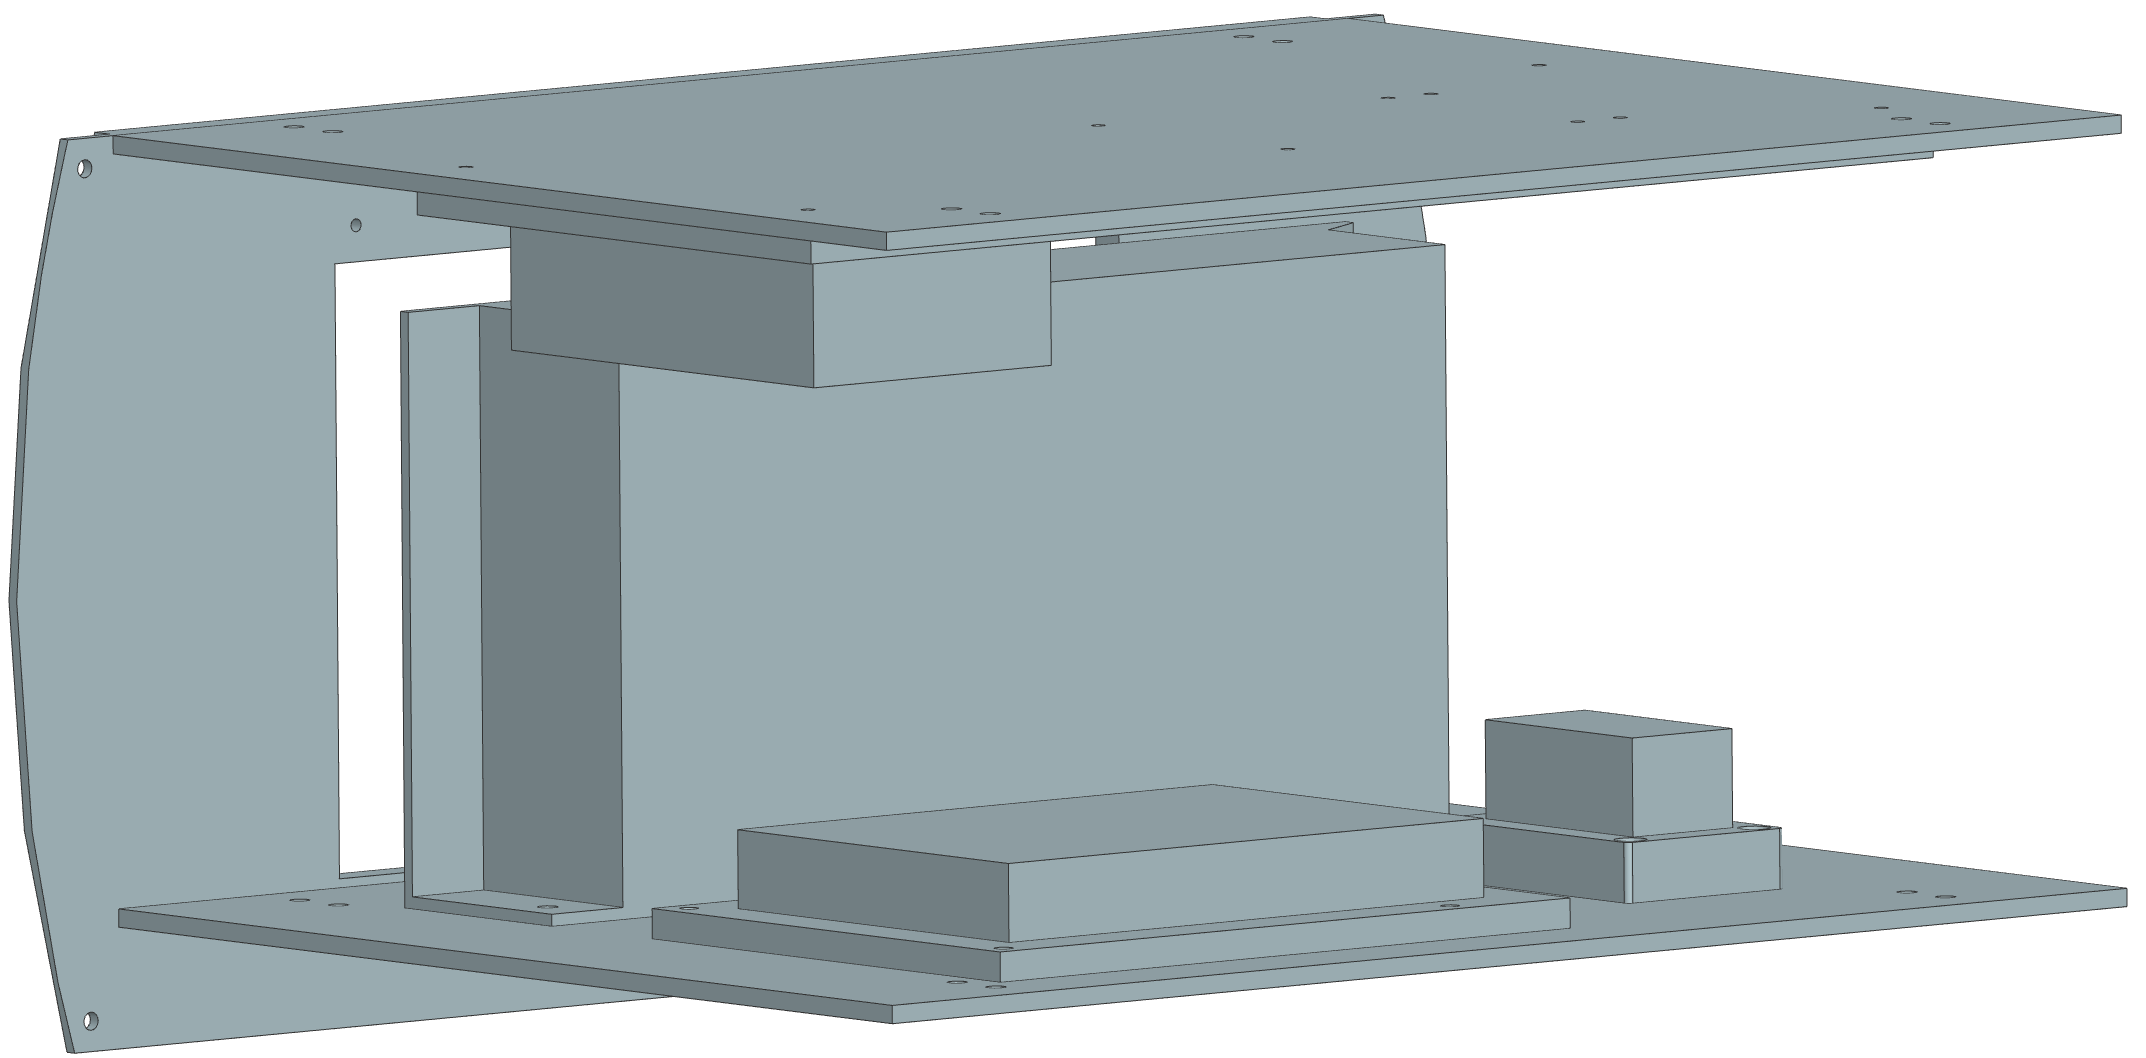
\includegraphics[scale=0.55]{98_images/assembly_controller_a_01.PNG}
    \caption{CAD-Modell des Gehäuses.}
    \label{fig:cad_modell_01}
\end{figure}

\begin{figure}[H]
    \centering
    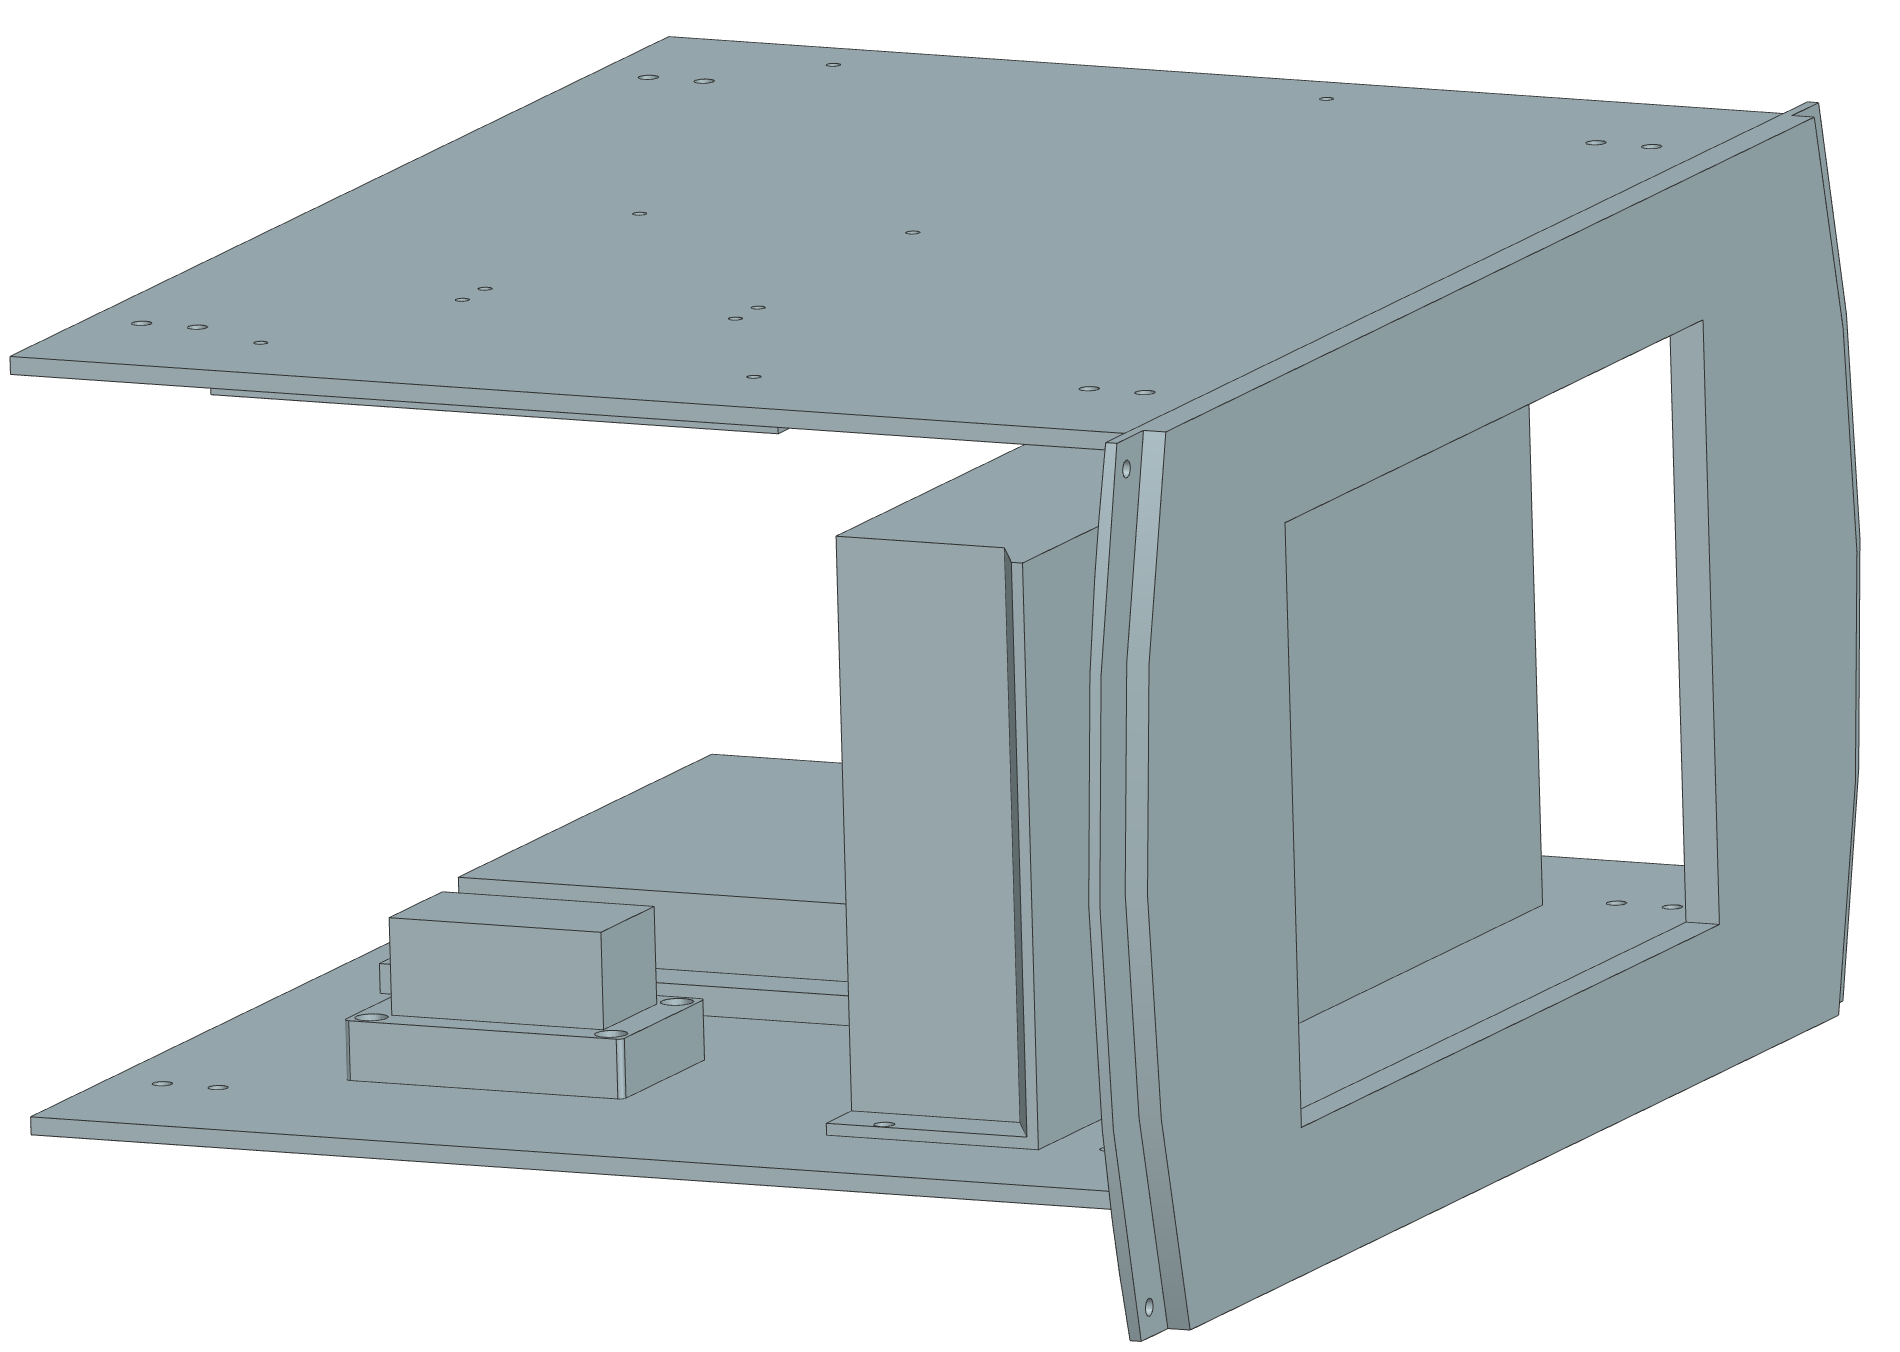
\includegraphics[scale=0.55]{98_images/assembly_controller_a_02.PNG}
    \caption{CAD-Modell des Gehäuses.}
    \label{fig:cad_modell_02}
\end{figure}

\subsection{Schema Pumpdiodenhalterung}
\label{chptr:_pumpdiodenhalterung}

\begin{figure}[H]
    \centering
    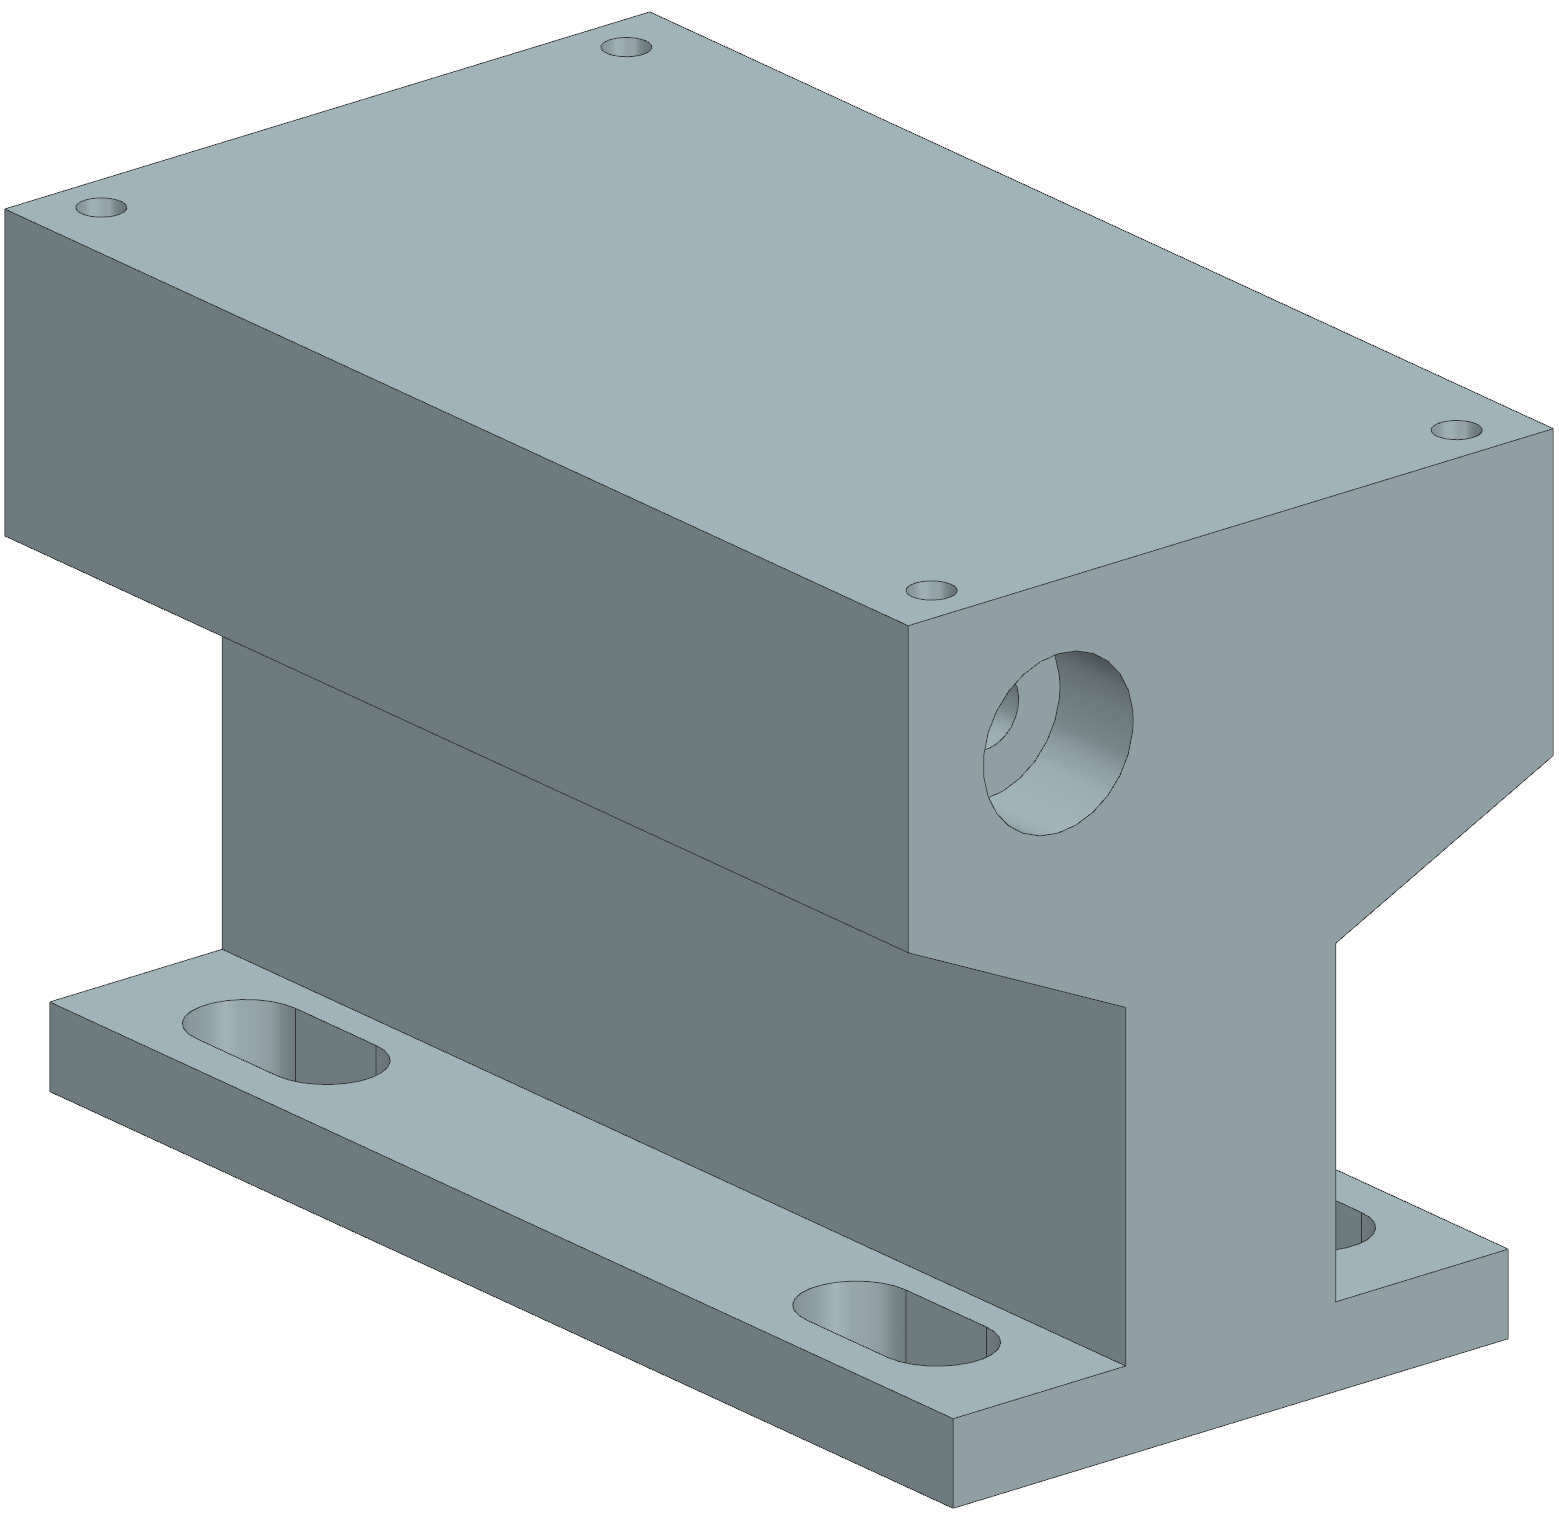
\includegraphics[scale=0.35]{98_images/kuehlblock_isometrie.PNG}
    \caption{Der gesamte Kühlblock.}
    \label{fig:enter-label}
\end{figure}

\begin{figure}[H]
    \centering
    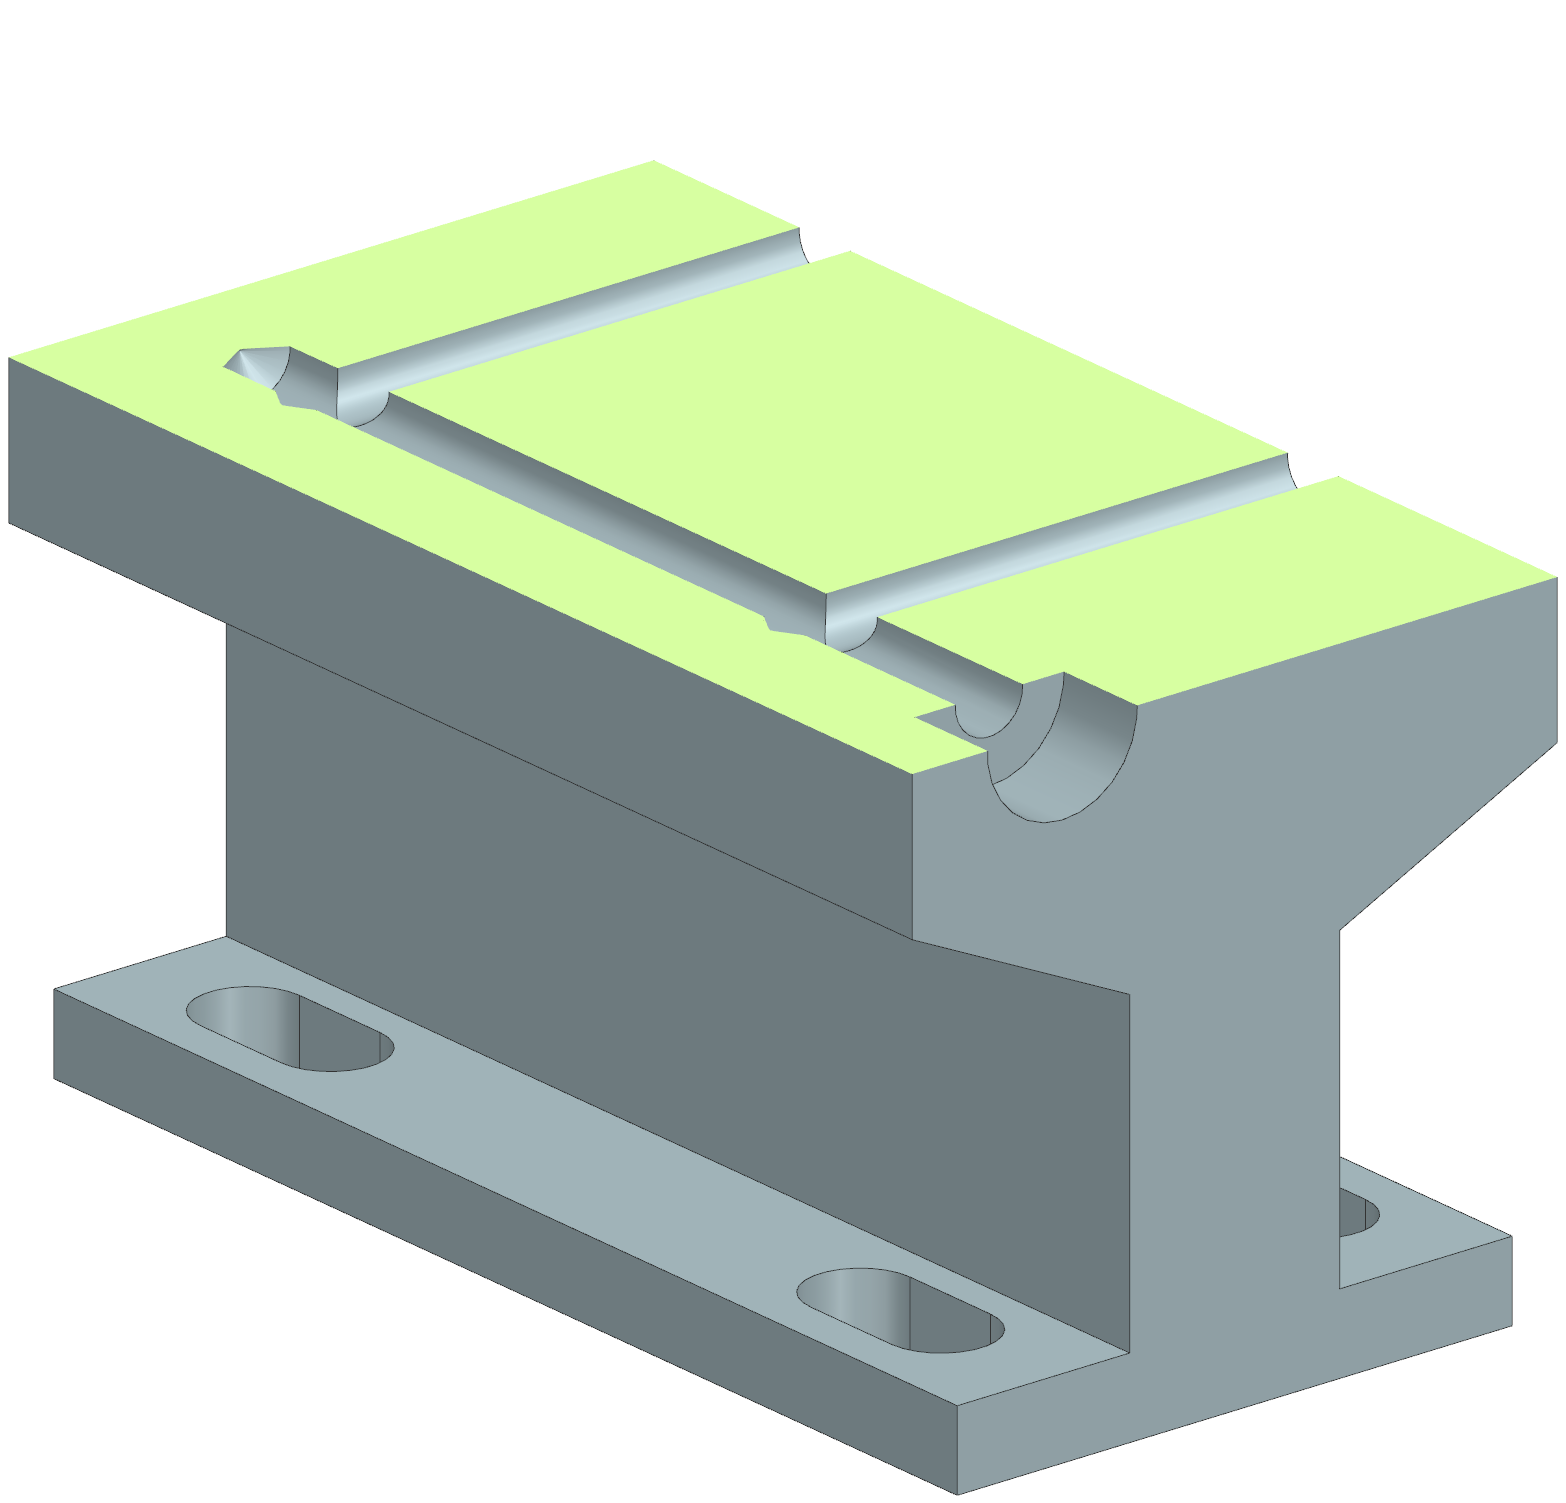
\includegraphics[scale=0.35]{98_images/kuehlblock_section.PNG}
    \caption{Der Kühlblock in der Schnittansicht zur Visualisierung der Wasserkanäle.}
    \label{fig:enter-label}
\end{figure}

\subsection{Elektroschemata der Komponenten}

\begin{figure}[H]
    \centering
    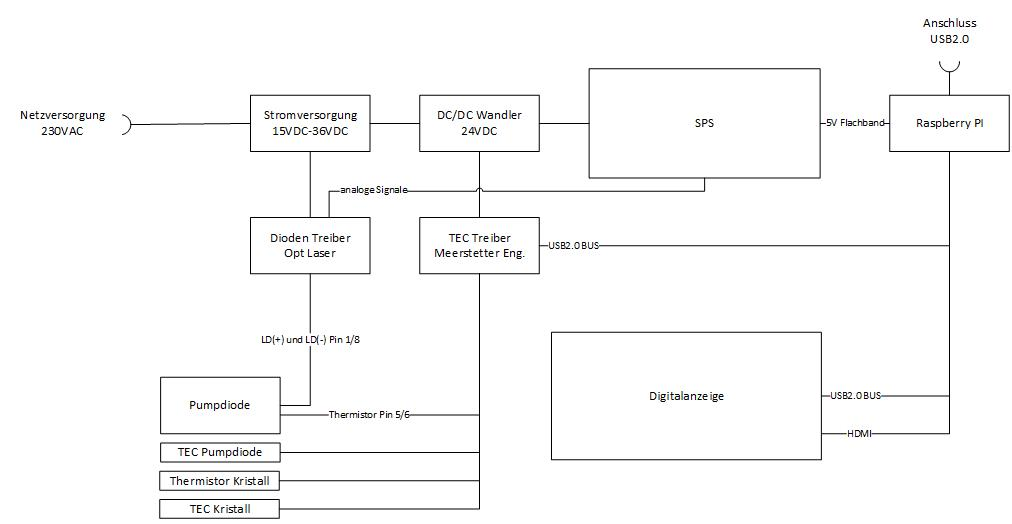
\includegraphics[scale=0.8, angle=90]{98_images/fhnw_pro6m_el_schema_overview.jpg}
    \caption{Überblick der elektrischen Verbindungen der gesamten Steuerung.}
    \label{fig:electric_overview}
\end{figure}

\clearpage

\begin{figure}[H]
    \centering
    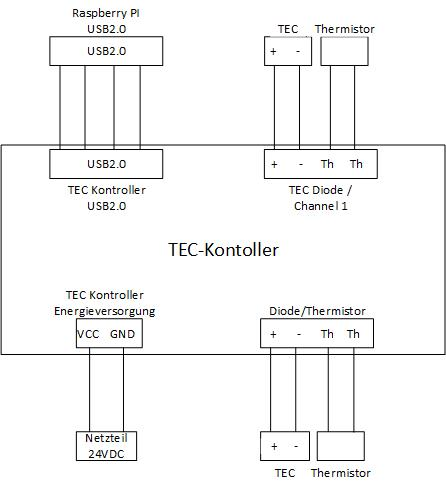
\includegraphics[scale=1.2, angle=90]{98_images/fhnw_pro6m_el_schema_tec.jpg}
    \caption{Überblick der elektrischen Verbindungen des TEC-Kontrollers.}
    \label{fig:electric_tec}
\end{figure}

\clearpage

\begin{figure}[H]
    \centering
    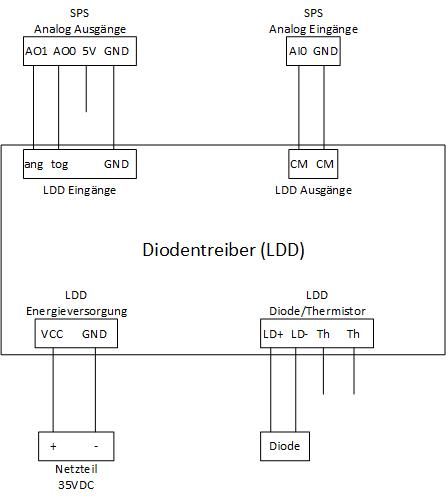
\includegraphics[scale=1.2, angle=90]{98_images/fhnw_pro6m_el_schema_ldd.jpg}
    \caption{Überblick der elektrischen Verbindungen des Diodentreibers.}
    \label{fig:electric_ldd}
\end{figure}

\clearpage

\subsection{Beschreibung einiger Drittanbieter-Bibliotheken für die Programmierung}

% \subsubsection{Queue}
% <<In computer science, a queue is a collection of entities that are maintained in a sequence and can be modified by the addition of entities at one end of the sequence and the removal of entities from the other end of the sequence.>> [] https://en.wikipedia.org/wiki/Queue_(abstract_data_type)

\subsubsection{Python Bibliothek - \textit{pandas}}
<<\textit{pandas} ist eine Programmbibliothek für Python zur Verarbeitung, Analyse und Darstellung von Daten. Insbesondere enthält sie Datenstrukturen und Operatoren für den Zugriff auf numerische Tabellen und Zeitreihen. \textit{pandas} ist Freie Software, veröffentlicht unter der 3-Klausel-BSD-Lizenz. Der Name leitet sich von dem englischen Begriff panel data (Paneldaten) ab, einer ökonometrischen Bezeichnung für Datensätze, die Beobachtungen über mehrere Zeiträume für dieselbe Untersuchungseinheit enthalten.>> [10]

\subsubsection{Python Bibliothek - \textit{NumPy}}
<<\textit{NumPy} ist eine Programmbibliothek für die Programmiersprache Python, die eine einfache Handhabung von Vektoren, Matrizen oder generell großen mehrdimensionalen Arrays ermöglicht. Neben den Datenstrukturen bietet \textit{NumPy} auch effizient implementierte Funktionen für numerische Berechnungen an.>> [11]

\subsection{Tests}
Die Tests für die TECs wurden mit der Software von Meerstetter getestet. Die Temperaturen wurden jedoch auf der Steuerung selber eingestellt. Erkennbar ist, dass die Temperaturen von 18°C bzw. 20°C gut angenähert werden, das Annähern unter Last jedoch nicht sehr effizient ist. Getestet wurden verschiedene Leistungen bei einer Kühlwassertemperatur von ca. 23.5°C. Der Kristall wurde im Labor nochmals auf dem Laser getestet und fest gestellt, dass der Einschwingvorgang nicht sehr effizient ist. Die PID-Parameter begrenzen die Effizienz beträchtlich, der maximal mögliche Leistung wird dadurch nicht bezogen.

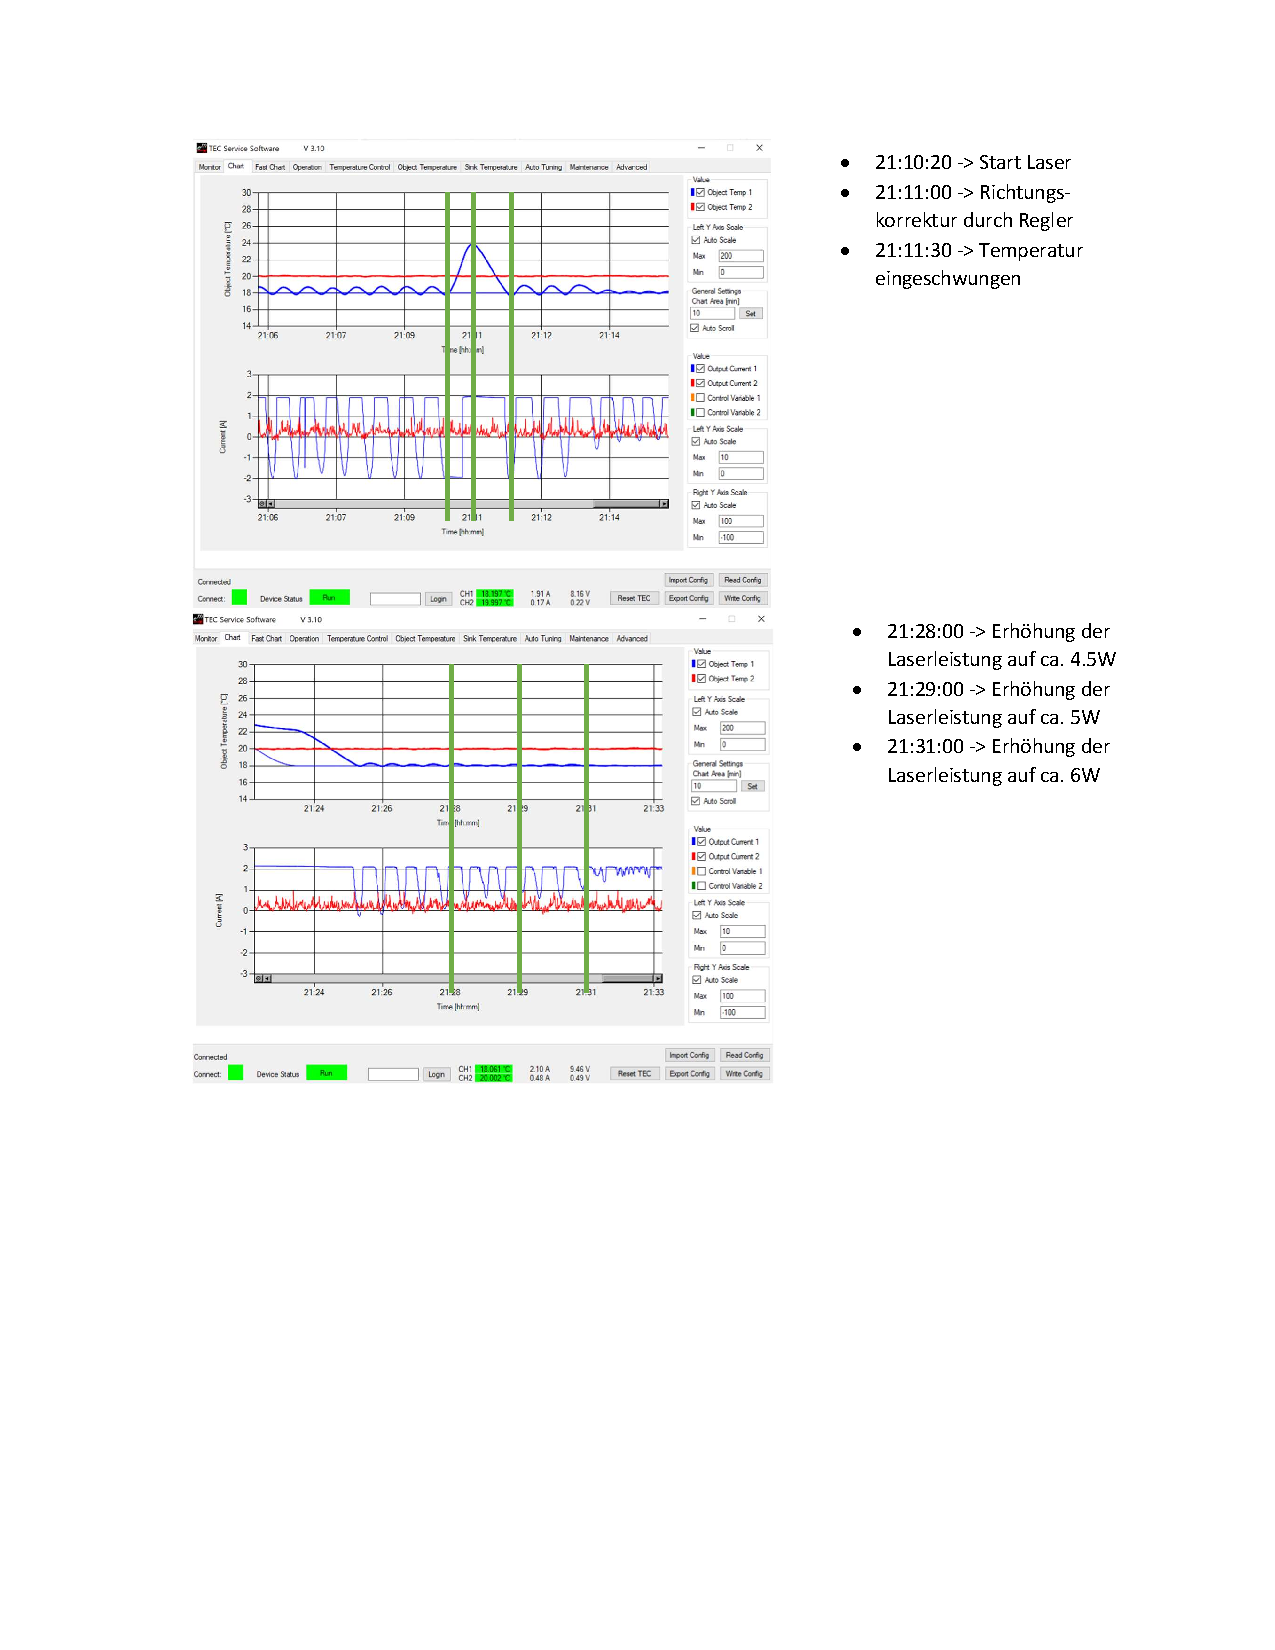
\includepdf[pages=1, scale=1, angle=0, pagecommand={
\label{TEC Tests}}]
{11_PDFs/fhnw_test_tec_01.pdf}
\begin{landscape}
    \subsection{Beschreibung der Quell-Codes}
\subsubsection{Beschreibung des Skriptes <<gui\_custom.py>>}

\begin{figure}[H]
    \centering
    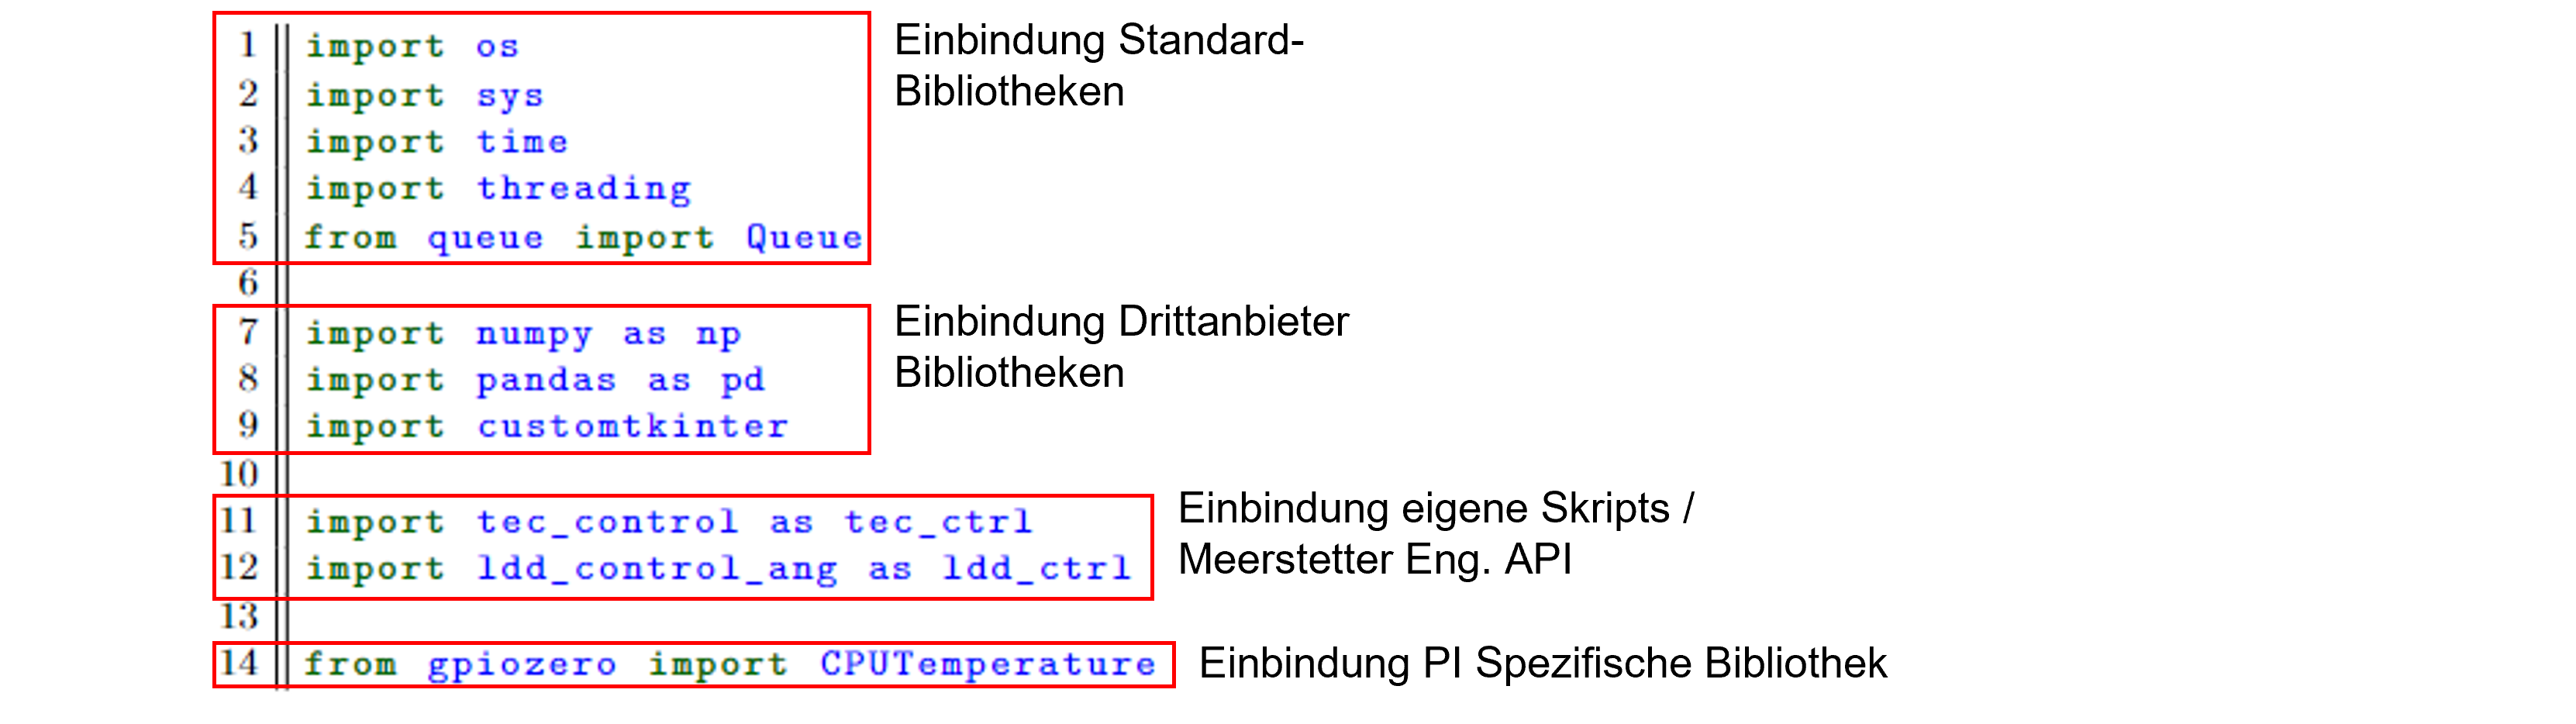
\includegraphics[scale=0.85]{98_images/src/fhnw_pro6m_quellcode_01.png}
    \caption*{Importierung erweiternder Bibliotheken}
    \label{fig:fhnw_pro6m_quellcode_01}
\end{figure}

\begin{figure}[H]
    \centering
    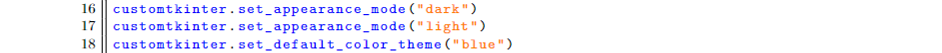
\includegraphics[scale=0.85]{98_images/src/fhnw_pro6m_quellcode_02.png}
    \caption*{Vorbelegung der Farbschemata für die Darstellung der GUI}
    \label{fig:fhnw_pro6m_quellcode_02}
\end{figure}

\begin{figure}[H]
    \centering
    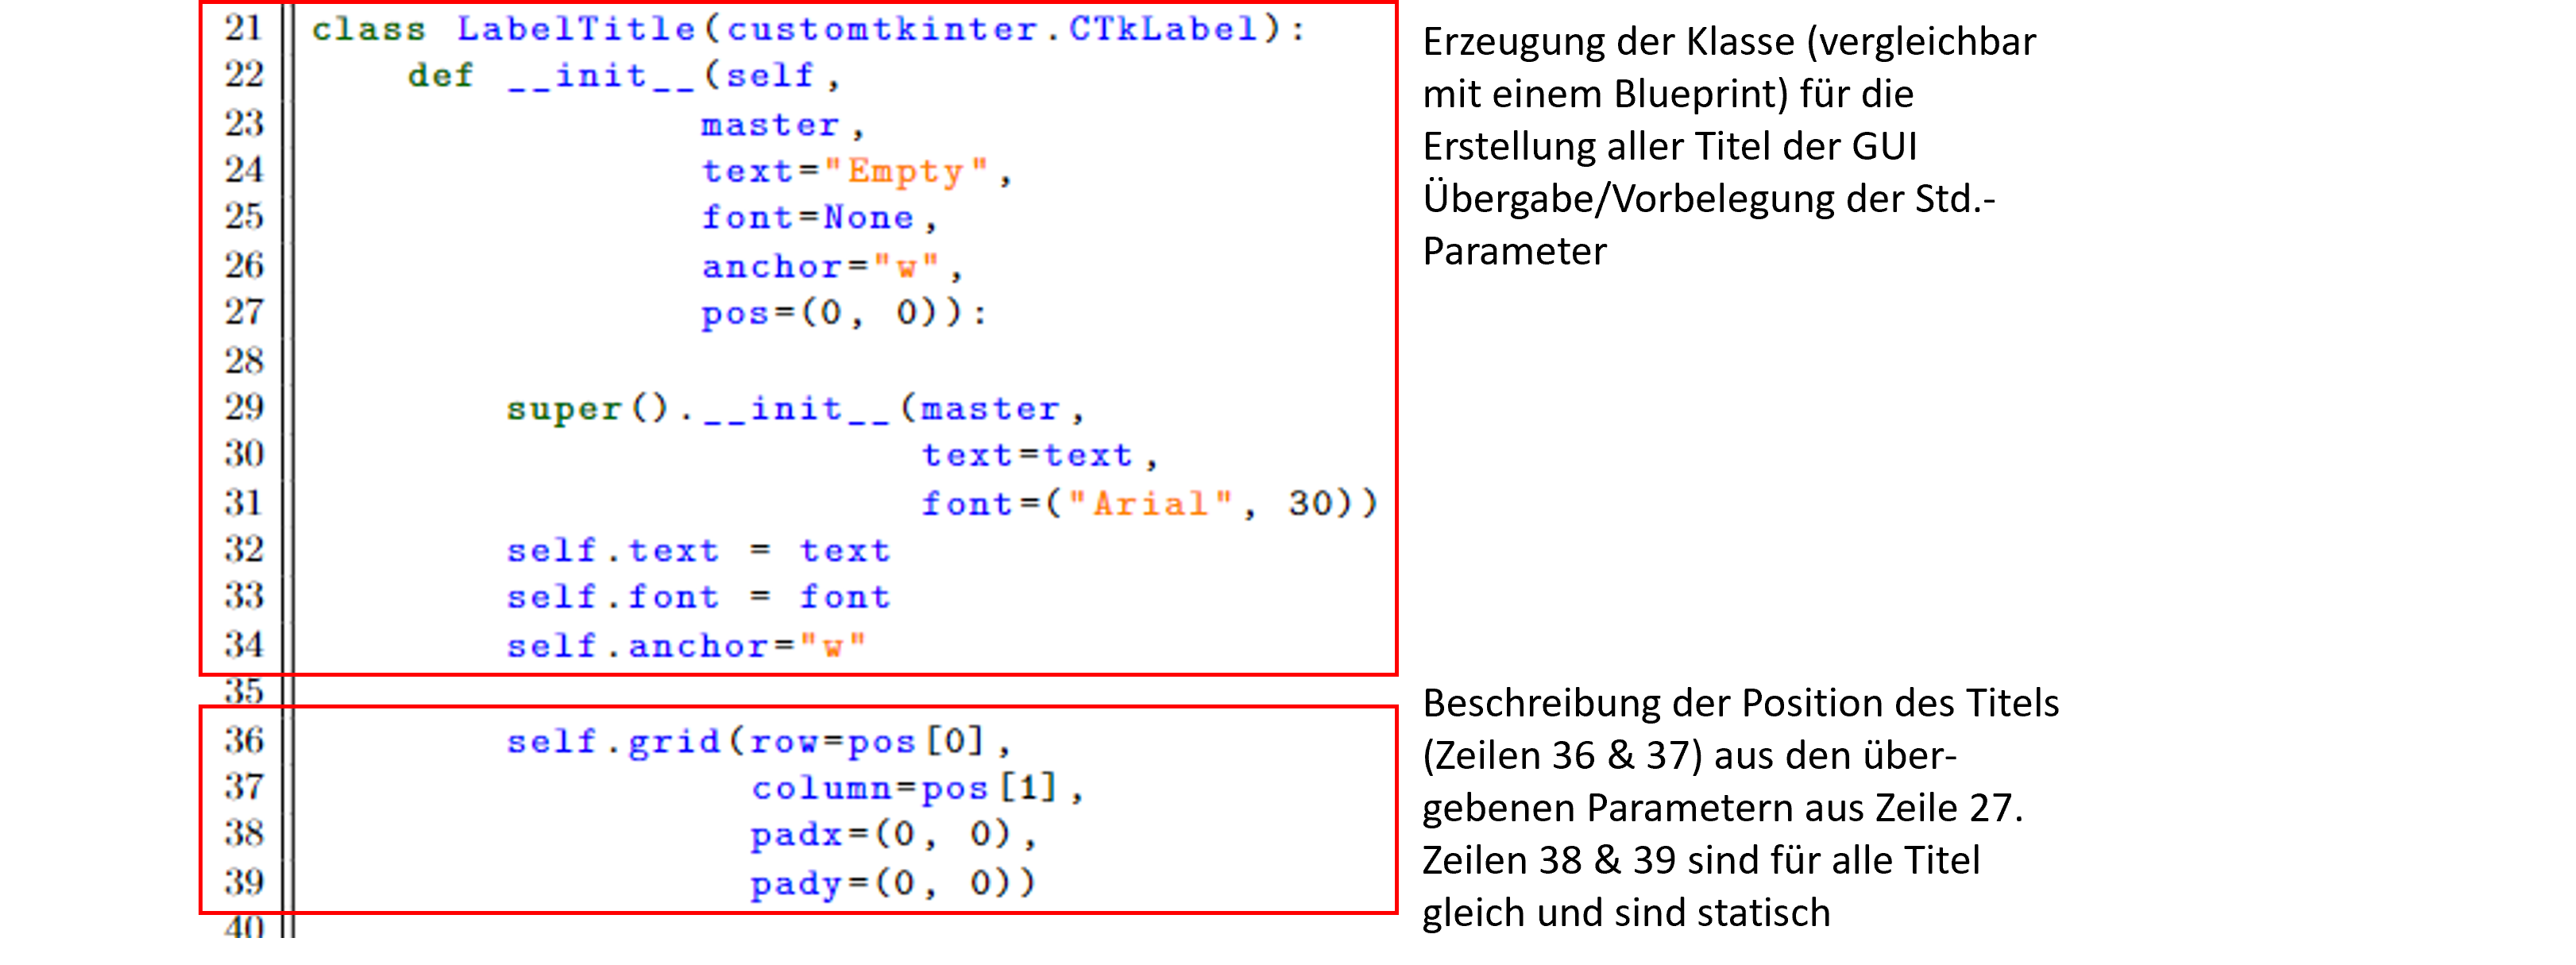
\includegraphics[scale=0.85]{98_images/src/fhnw_pro6m_quellcode_03.png}
    \caption*{Erstellung der Klasse für die Titel der Benutzeroberfläche}
    \label{fig:fhnw_pro6m_quellcode_03}
\end{figure}

\begin{figure}[H]
    \centering
    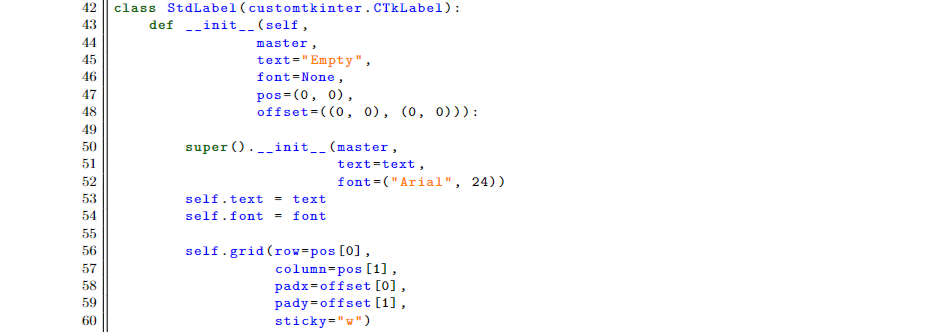
\includegraphics[scale=0.85]{98_images/src/fhnw_pro6m_quellcode_04.png}
    \caption*{Erstellung der Klasse für sämtliche Texte der Benutzeroberfläche}
    \label{fig:fhnw_pro6m_quellcode_04}
\end{figure}

\begin{figure}[H]
    \centering
    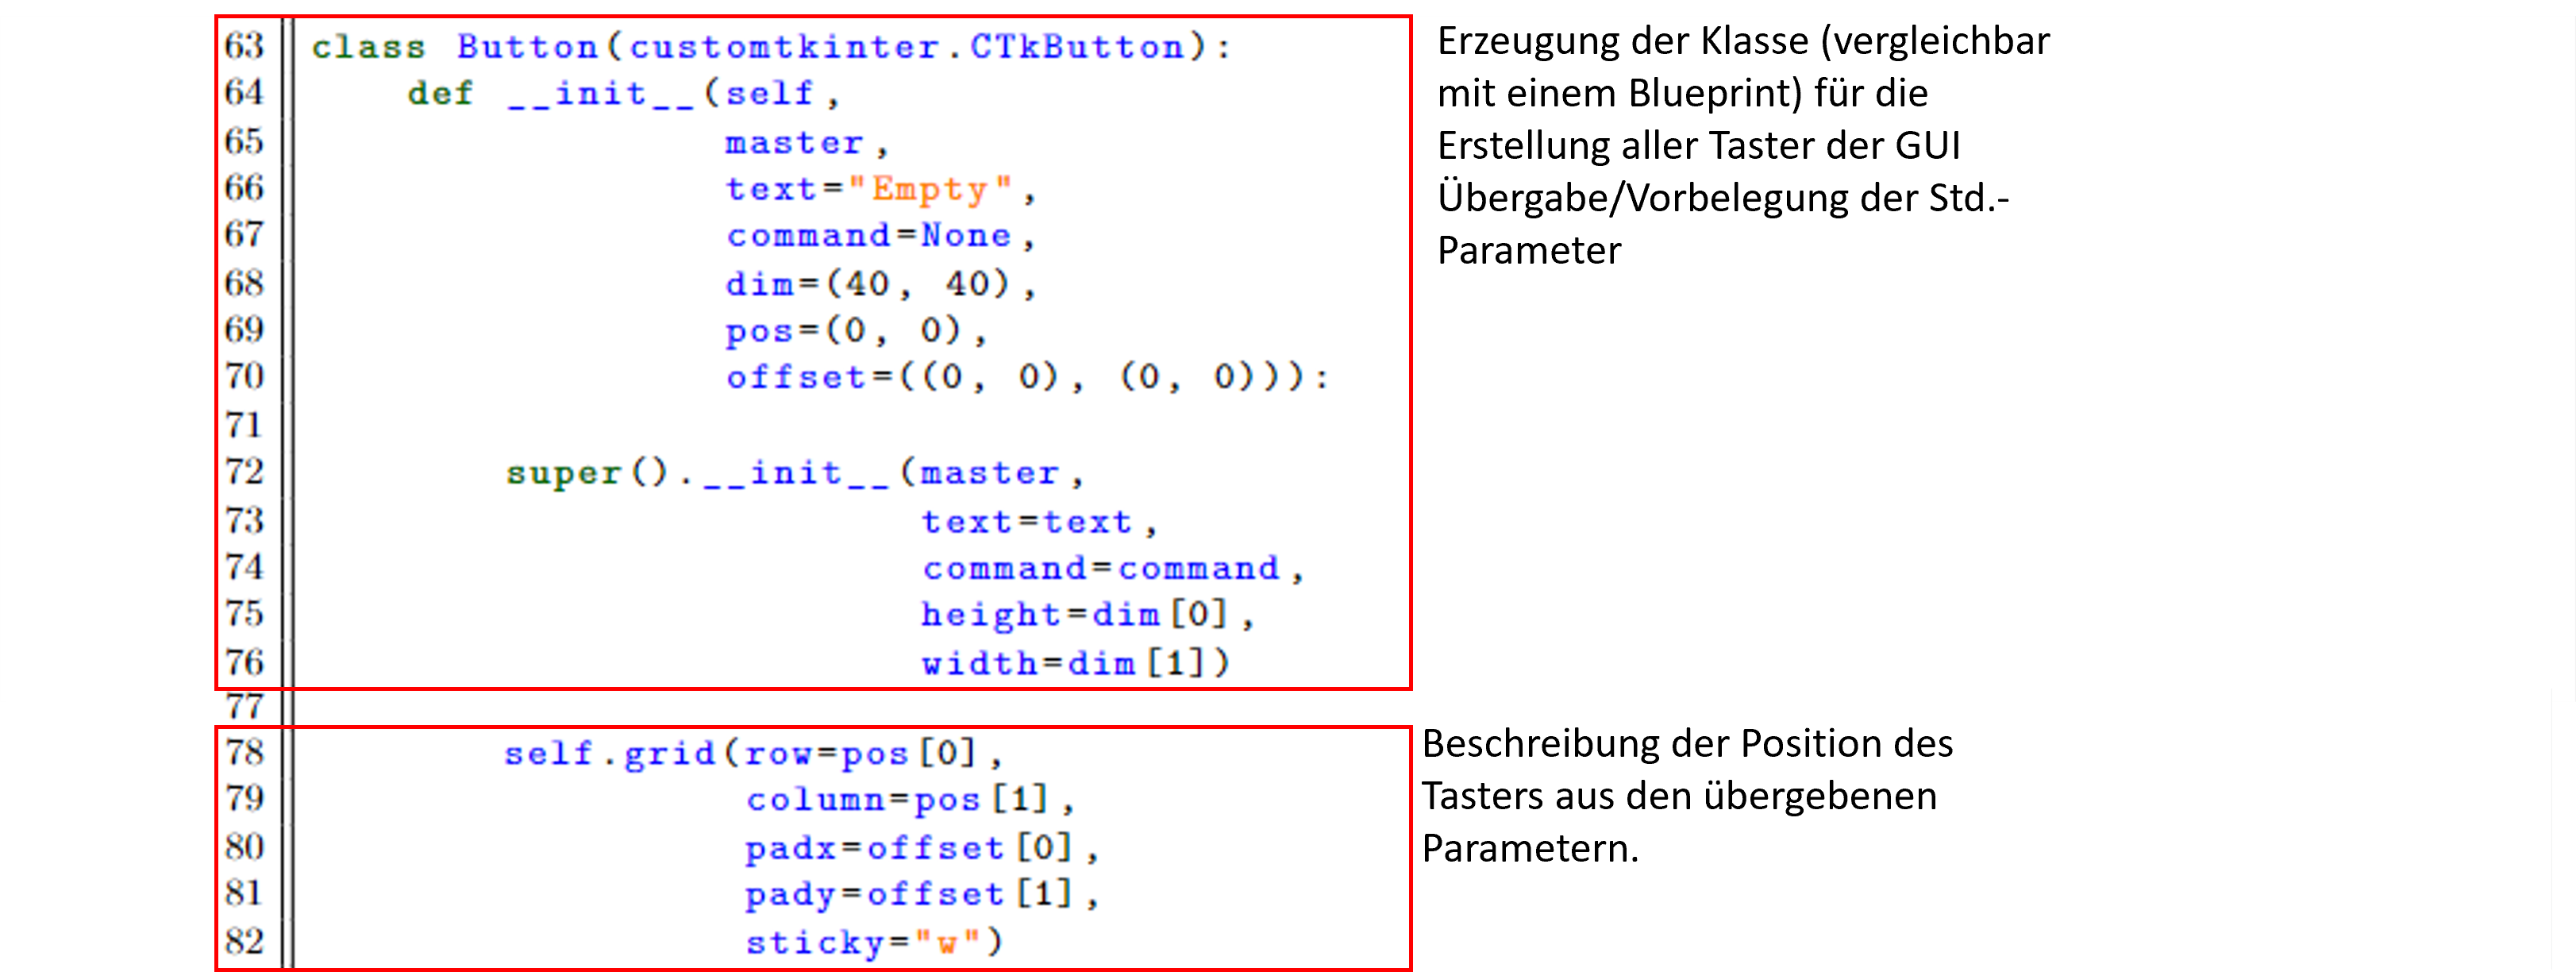
\includegraphics[scale=0.85]{98_images/src/fhnw_pro6m_quellcode_05.png}
    \caption{Erstellung der Klasse für die Taster der Benutzeroberfläche}
    \label{fig:fhnw_pro6m_quellcode_05}
\end{figure}

\begin{figure}[H]
    \centering
    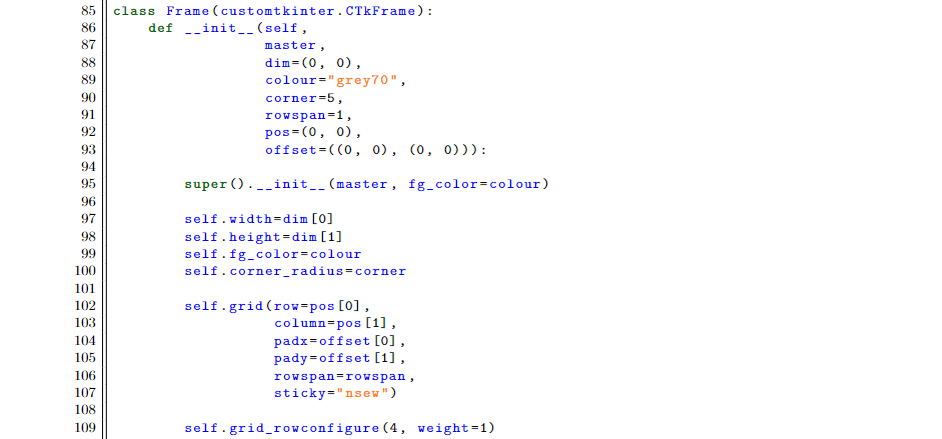
\includegraphics[scale=0.85]{98_images/src/fhnw_pro6m_quellcode_06.png}
    \caption{Erstellung der Klasse für sämtliche Rahmen der Benutzeroberfläche}
    \label{fig:fhnw_pro6m_quellcode_06}
\end{figure}

\begin{figure}[H]
    \centering
    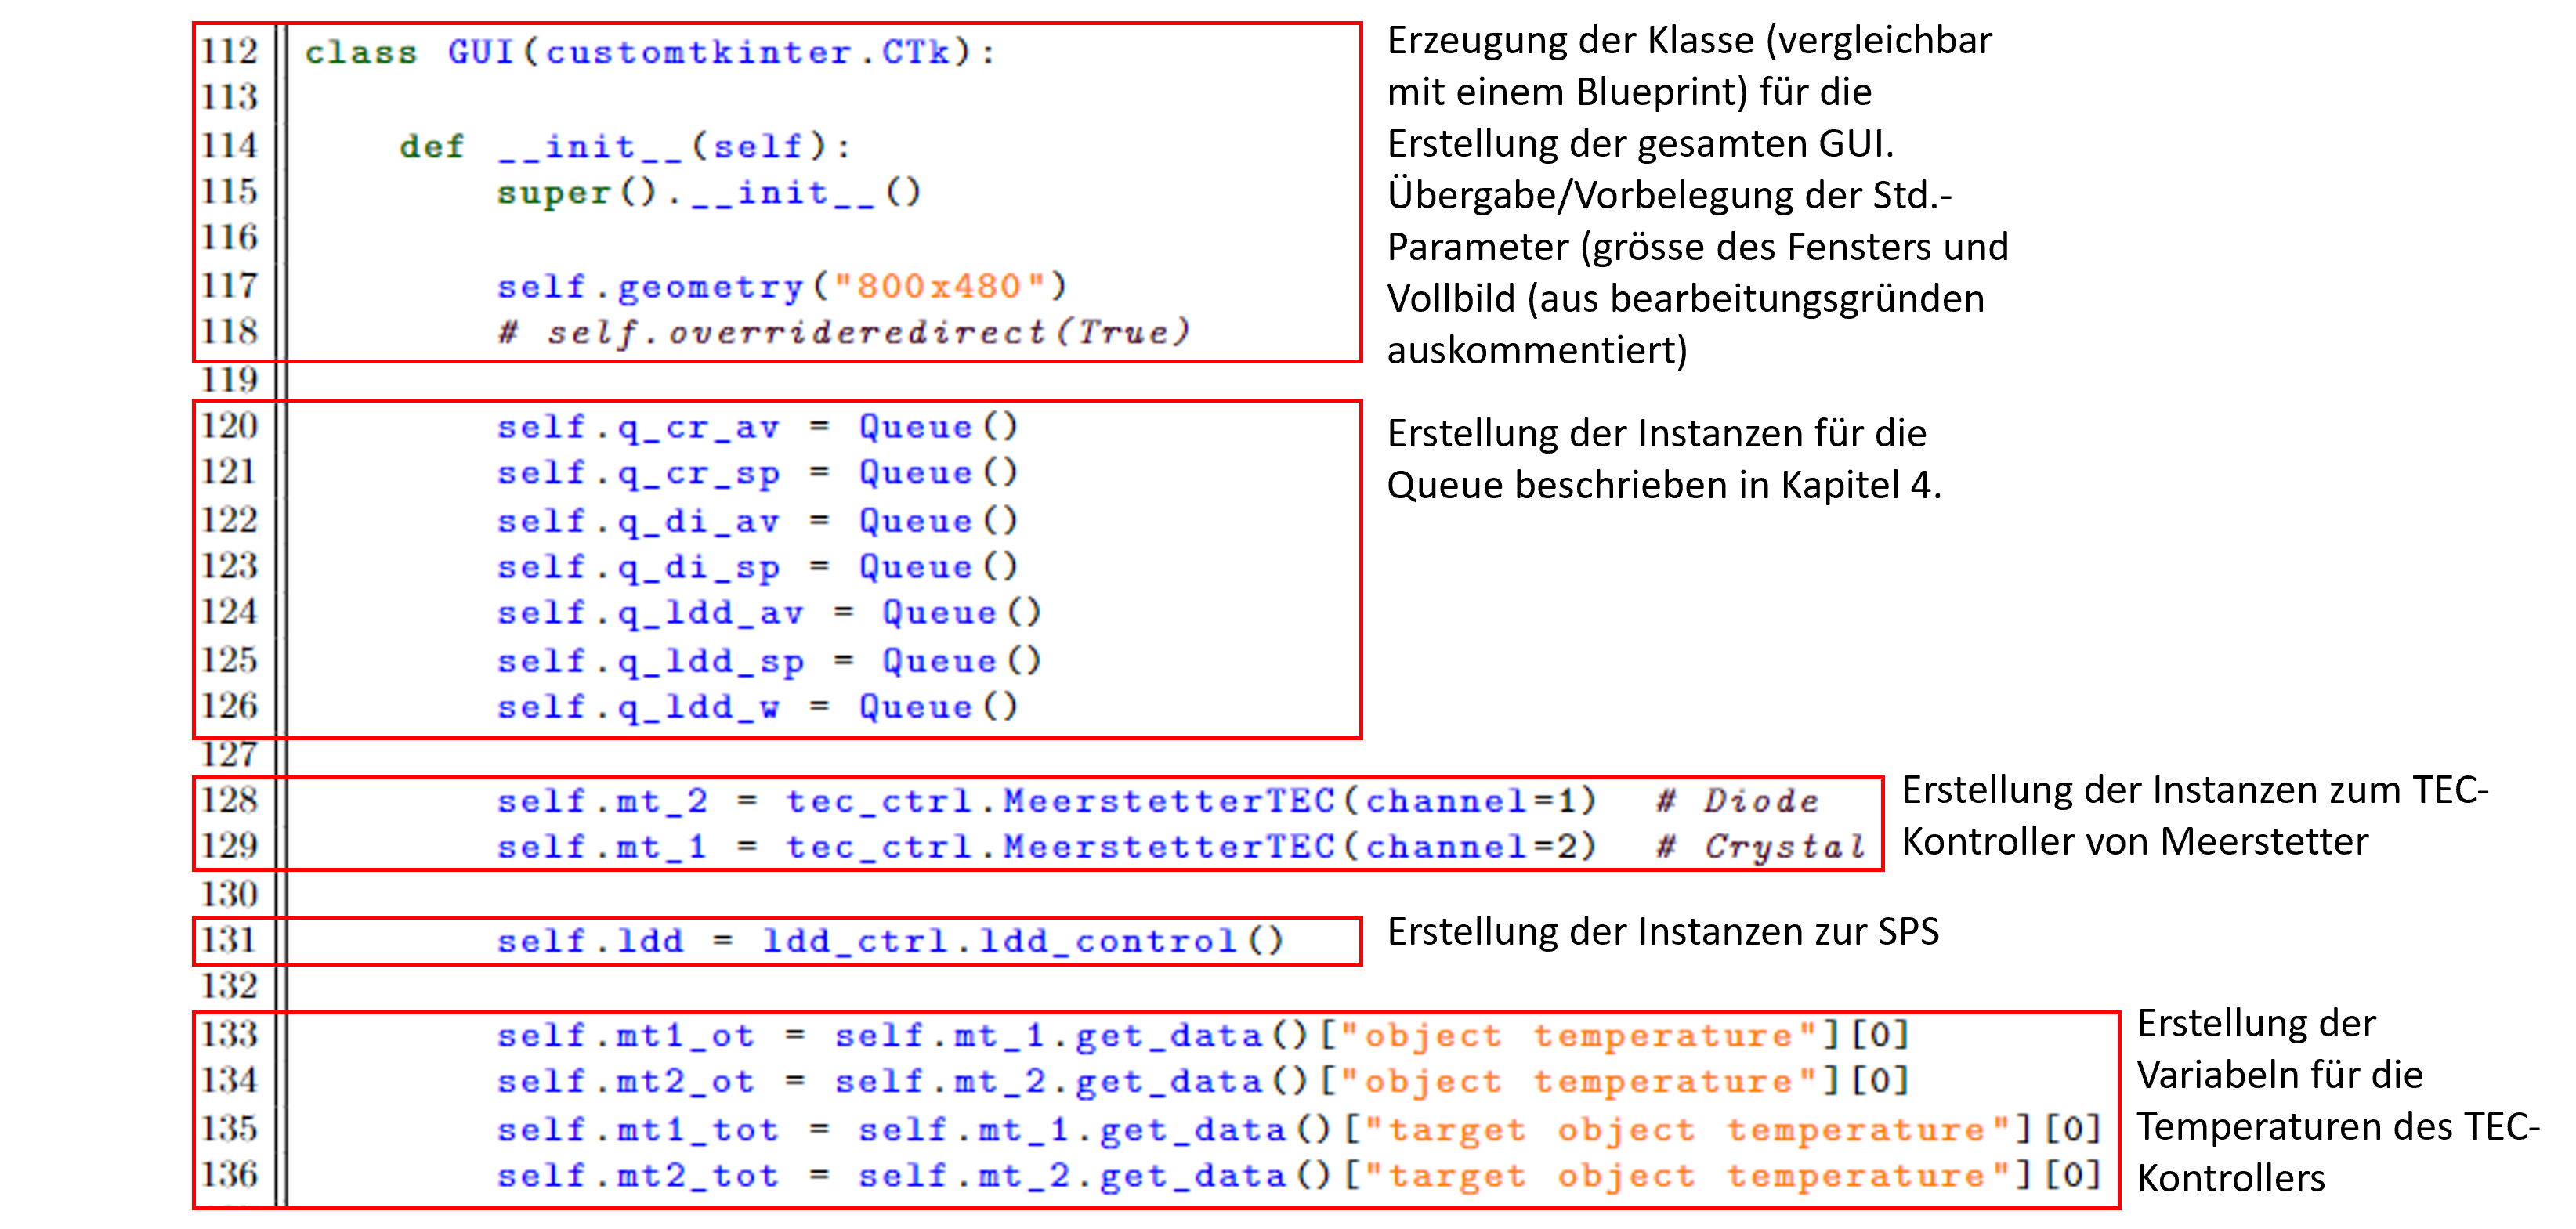
\includegraphics[scale=0.7]{98_images/src/fhnw_pro6m_quellcode_07.png}
    \caption{Erstellung der Hauptklasse für die gesamte Benutzeroberfläche der Benutzeroberfläche. Alle in der Benutzeroberfläche global genutzte Variablen werden in der Funktion <<def __init__(self):>> definiert. Aus dem Grund der Objektorientierung werden die Variablen mit dem Wort <<self.>> definiert. Es referenziert auf die Klasseninstanz in der sie definiert worden ist.}
    \label{fig:fhnw_pro6m_quellcode_07}
\end{figure}

\begin{figure}[H]
    \centering
    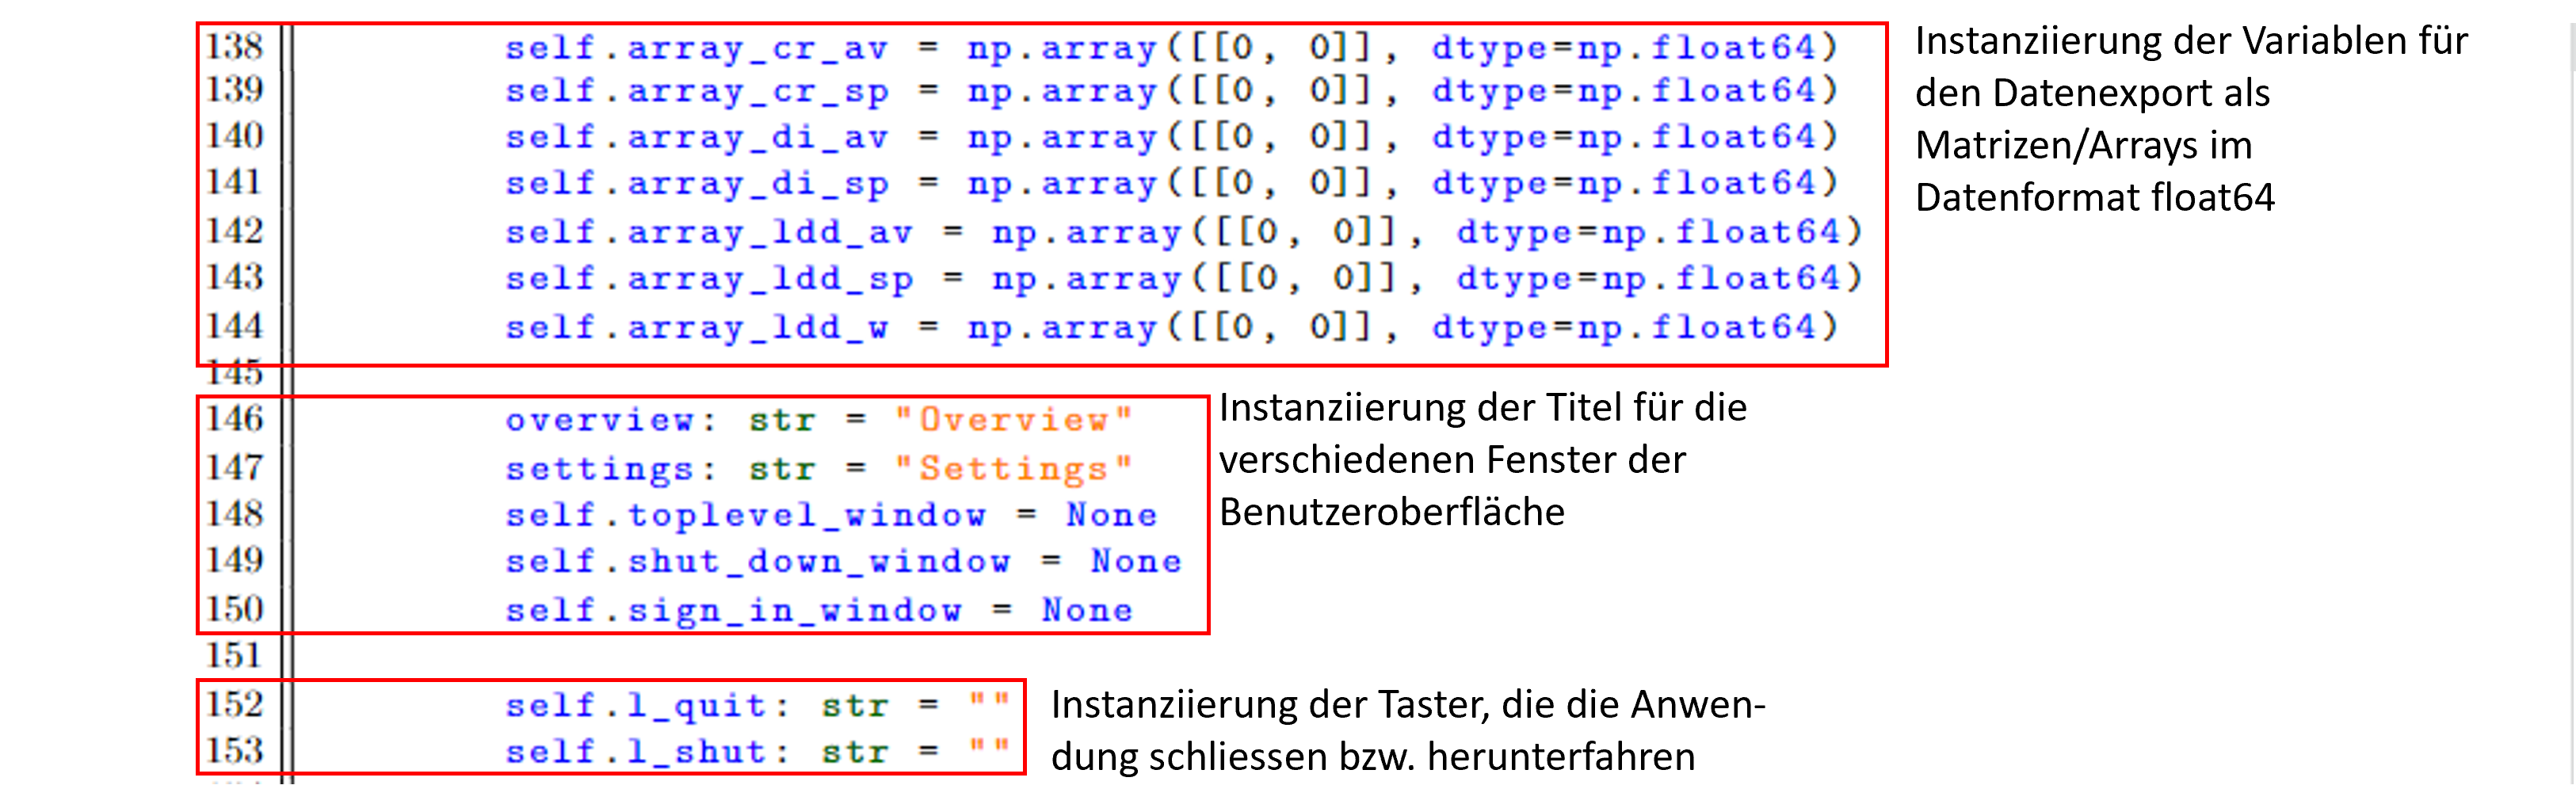
\includegraphics[scale=0.75, trim= 1mm 1mm 1mm 1mm, clip]{98_images/src/fhnw_pro6m_quellcode_08.png}
    \caption{Weiter globale Variablen.}
    \label{fig:fhnw_pro6m_quellcode_08}
\end{figure}

\begin{figure}[H]
    \centering
    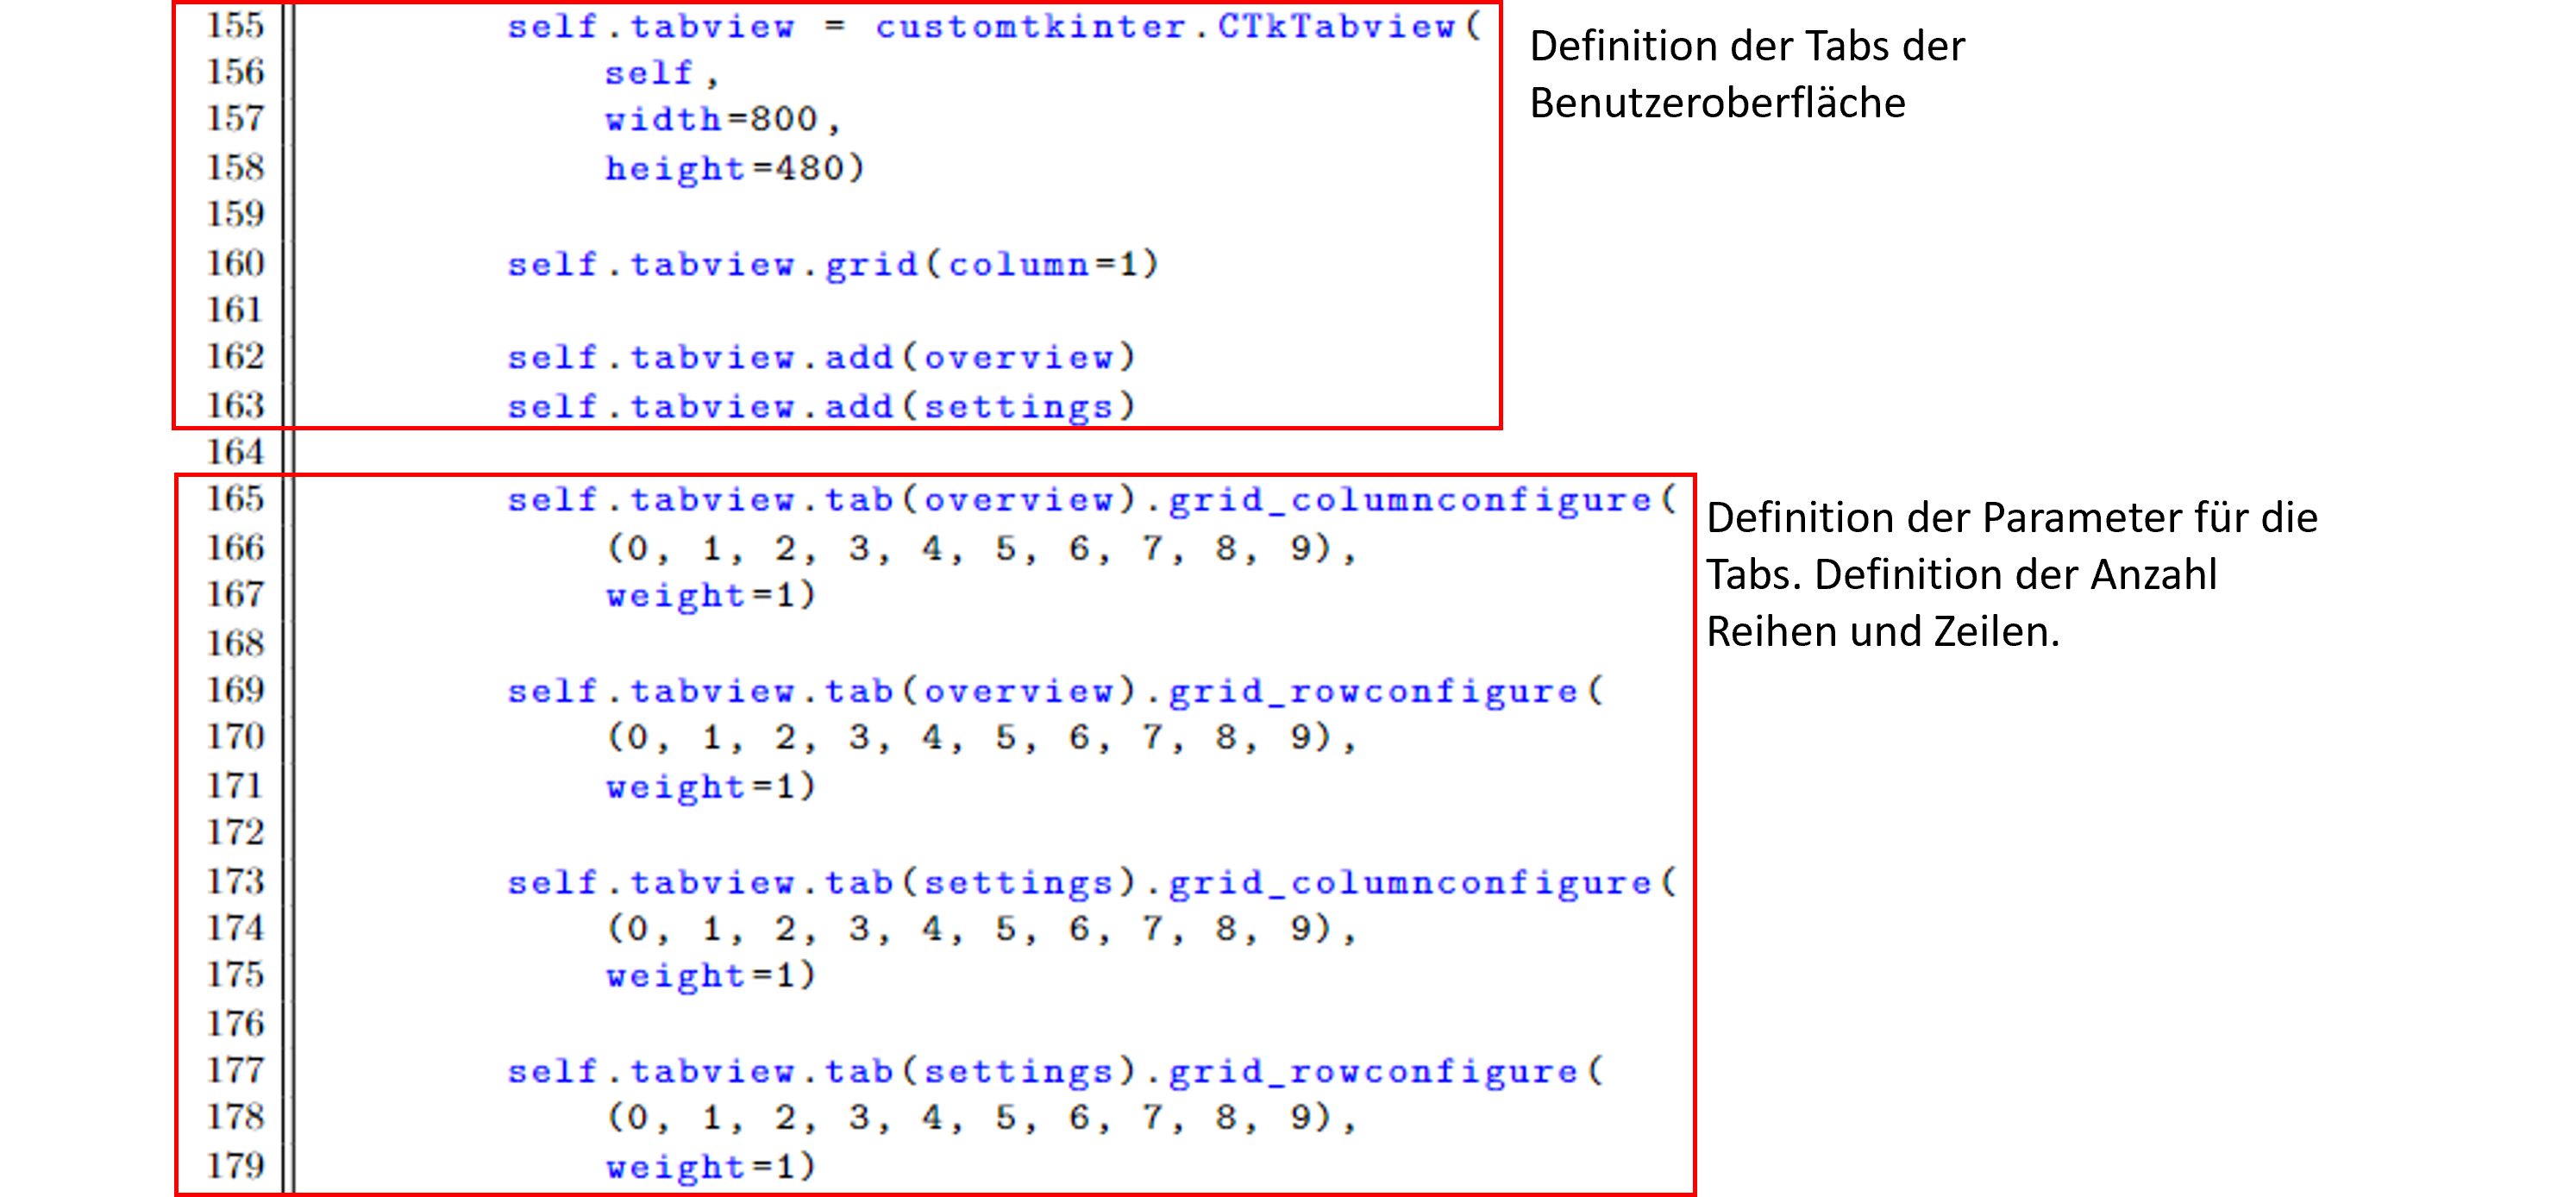
\includegraphics[scale=0.75]{98_images/src/fhnw_pro6m_quellcode_09.png}
    \caption*{Instanziierung der Tabs der Benutzeroberfläche <<Overview>> und <<Settings>>.}
    \label{fig:fhnw_pro6m_quellcode_09}
\end{figure}

\begin{figure}[H]
    \centering
    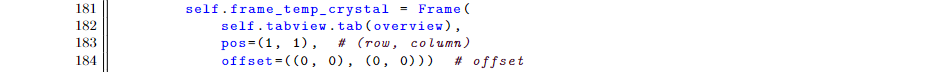
\includegraphics[scale=0.8]{98_images/src/fhnw_pro6m_quellcode_10.png}
    \caption*{Ein Beispiel für die Instanziierung für einen Rahmen. Alle Rahmen der GUI wurden nach exakt diesem Schema erstellt und wird aus diesem Grund nur einmal erläutert.}
    \label{fig:fhnw_pro6m_quellcode_10}
\end{figure}

\begin{figure}[H]
    \centering
    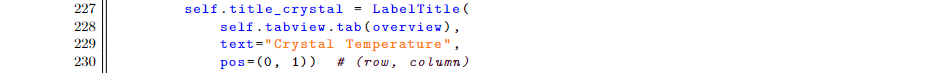
\includegraphics[scale=0.8]{98_images/src/fhnw_pro6m_quellcode_11.png}
    \caption*{Ein Beispiel für die Erstellung eines Titels. Alle Titel der GUI wurden mit Hilfe der Klasse <<LabelTitel>> erstellt und sind aus diesem Grund alle identisch und wird aus diesem Grund nur einmal erläutert.}
    \label{fig:fhnw_pro6m_quellcode_11}
\end{figure}

\begin{figure}[H]
    \centering
    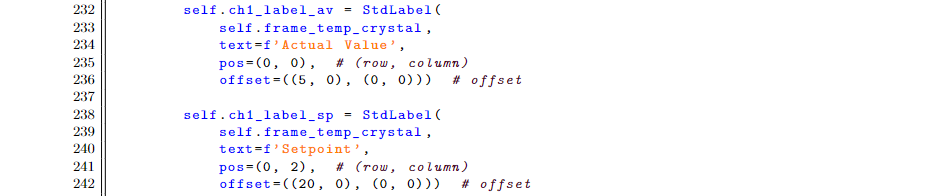
\includegraphics[scale=0.8]{98_images/src/fhnw_pro6m_quellcode_12.png}
    \caption*{Ein Beispiel für die Erstellung eines Textes. Alle Texte der GUI wurden mit Hilfe der Klasse <<StdLabel>> erstellt und sind aus diesem Grund alle identisch und wird aus diesem Grund nur jeweils für die Aktuellen und Werte und die Setpoints erläutert.}
    \label{fig:fhnw_pro6m_quellcode_12}
\end{figure}

\begin{figure}[H]
    \centering
    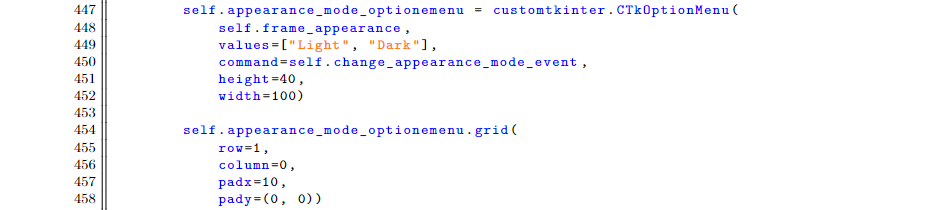
\includegraphics[scale=0.8]{98_images/src/fhnw_pro6m_quellcode_13.png}
    \caption*{Erstellung des Optionmenüs mit <<Drop-Down>>-Liste. Aus dem Grund des einmaligen Auftretens wurde dafür keine eigene Klasse erstellt.}
    \label{fig:fhnw_pro6m_quellcode_13}
\end{figure}

\begin{figure}[H]
    \centering
    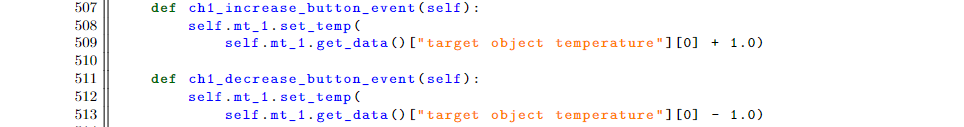
\includegraphics[scale=0.8]{98_images/src/fhnw_pro6m_quellcode_15.png}
    \caption*{Die Abgebildeten Funktionen können die Solltemperaturen hoch oder herunter gesetzt werden. Die Funktionen für die Temperaturen und die Stromstärke des Lasers sind sehr ähnlich. Aus diesem Grund wird nur eine der drei dargestellt.}
    \label{fig:fhnw_pro6m_quellcode_15}
\end{figure}

\begin{figure}[H]
    \centering
    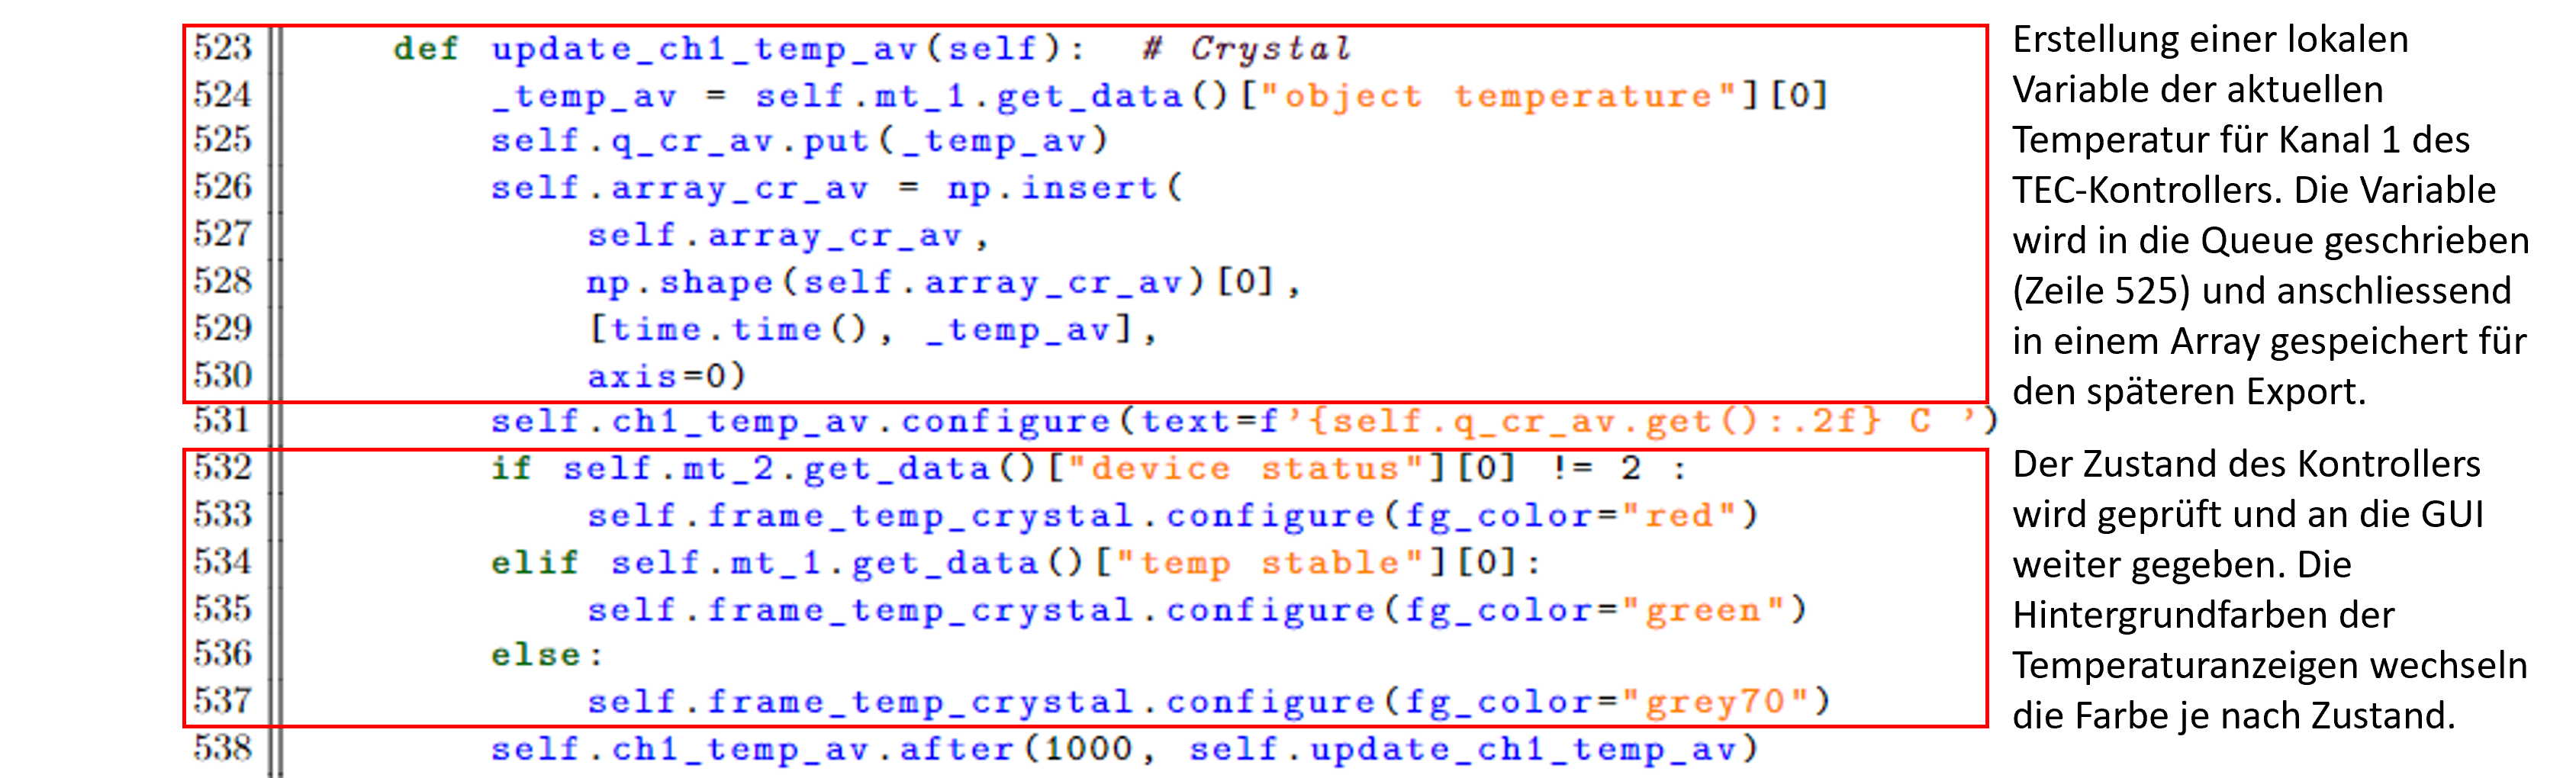
\includegraphics[scale=0.8]{98_images/src/fhnw_pro6m_quellcode_16.png}
    \caption*{Das Updaten der aktuellen und Sollwerte für sowohl die Temperaturen. Die Funktionen für die Temperaturen und die Stromstärke des Lasers sind sehr ähnlich. Aus diesem Grund wird nur eine der sechs dargestellt.}
    \label{fig:fhnw_pro6m_quellcode_16}
\end{figure}

\begin{figure}[H]
    \centering
    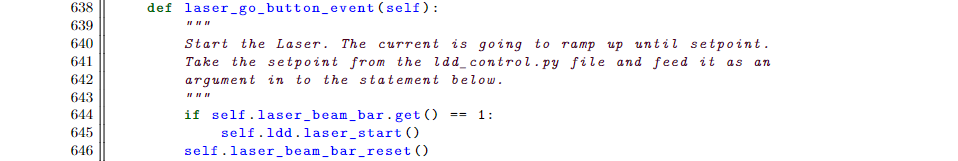
\includegraphics[scale=0.8]{98_images/src/fhnw_pro6m_quellcode_17.png}
    \caption*{Diese Funktion prüft und kontrolliert den Status des <<Enable>>-Tasters für das Starten des Lasers.}
    \label{fig:fhnw_pro6m_quellcode_17}
\end{figure}

\begin{figure}[H]
    \centering
    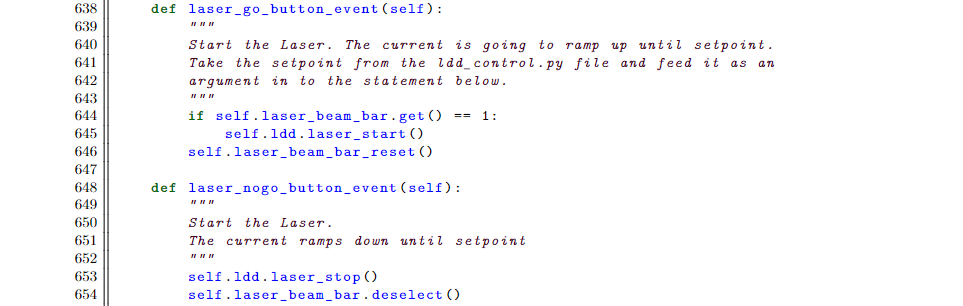
\includegraphics[scale=0.8]{98_images/src/fhnw_pro6m_quellcode_18.png}
    \caption*{Diese Funktion steuert das Starten bzw. das Beenden des Lasers. Vor dem Start werden Konditionen geprüft. Der Laser wird gestartet indem dem <<ldd\_controll.py>>-Skript Funktionen bezogen werden. (Zeile 645 bzw. 653)}
    \label{fig:fhnw_pro6m_quellcode_18}
\end{figure}

\begin{figure}[H]
    \centering
    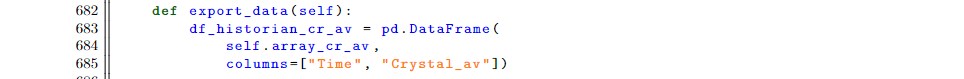
\includegraphics[scale=0.8]{98_images/src/fhnw_pro6m_quellcode_19.png}
    \caption*{Die Funktion erstellt aus den zuvor erstellten Arrays der aktuellen Wert und Setpoints pandas-Tabellen. Dies wurde lediglich einmal dargestellt, weil dies für alle Arrays gleich funktioniert.}
    \label{fig:fhnw_pro6m_quellcode_19}
\end{figure}

\begin{figure}[H]
    \centering
    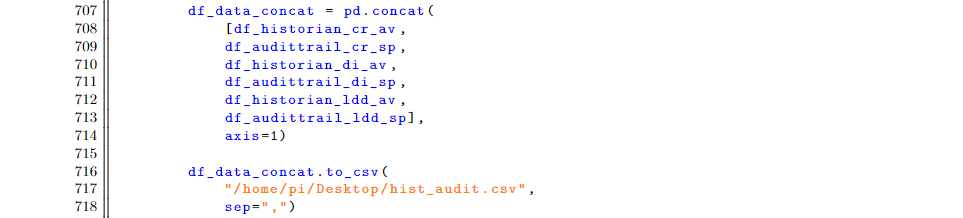
\includegraphics[scale=0.8]{98_images/src/fhnw_pro6m_quellcode_20.png}
    \caption*{Die in der selben Funktion gesammelten, einzelnen pandas-Tabellen werden zu einer grossen verscholzen und in den definierten Ôrdner exportiert.}
    \label{fig:fhnw_pro6m_quellcode_20}
\end{figure}

\begin{figure}[H]
    \centering
    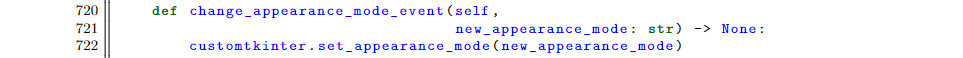
\includegraphics[scale=0.8]{98_images/src/fhnw_pro6m_quellcode_21.png}
    \caption*{Die Funktion zum anpassen des \textit{Dark}- und \textit{Light}-Modes der Benutzeroberfläche.}
    \label{fig:fhnw_pro6m_quellcode_21}
\end{figure}

\begin{figure}[H]
    \centering
    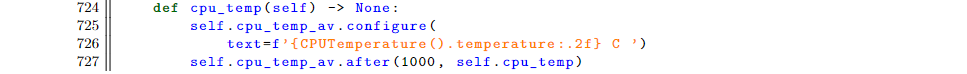
\includegraphics[scale=0.8]{98_images/src/fhnw_pro6m_quellcode_22.png}
    \caption*{Funktion zum Bezug der CPU Temperatur}
    \label{fig:fhnw_pro6m_quellcode_22}
\end{figure}

\begin{figure}[H]
    \centering
    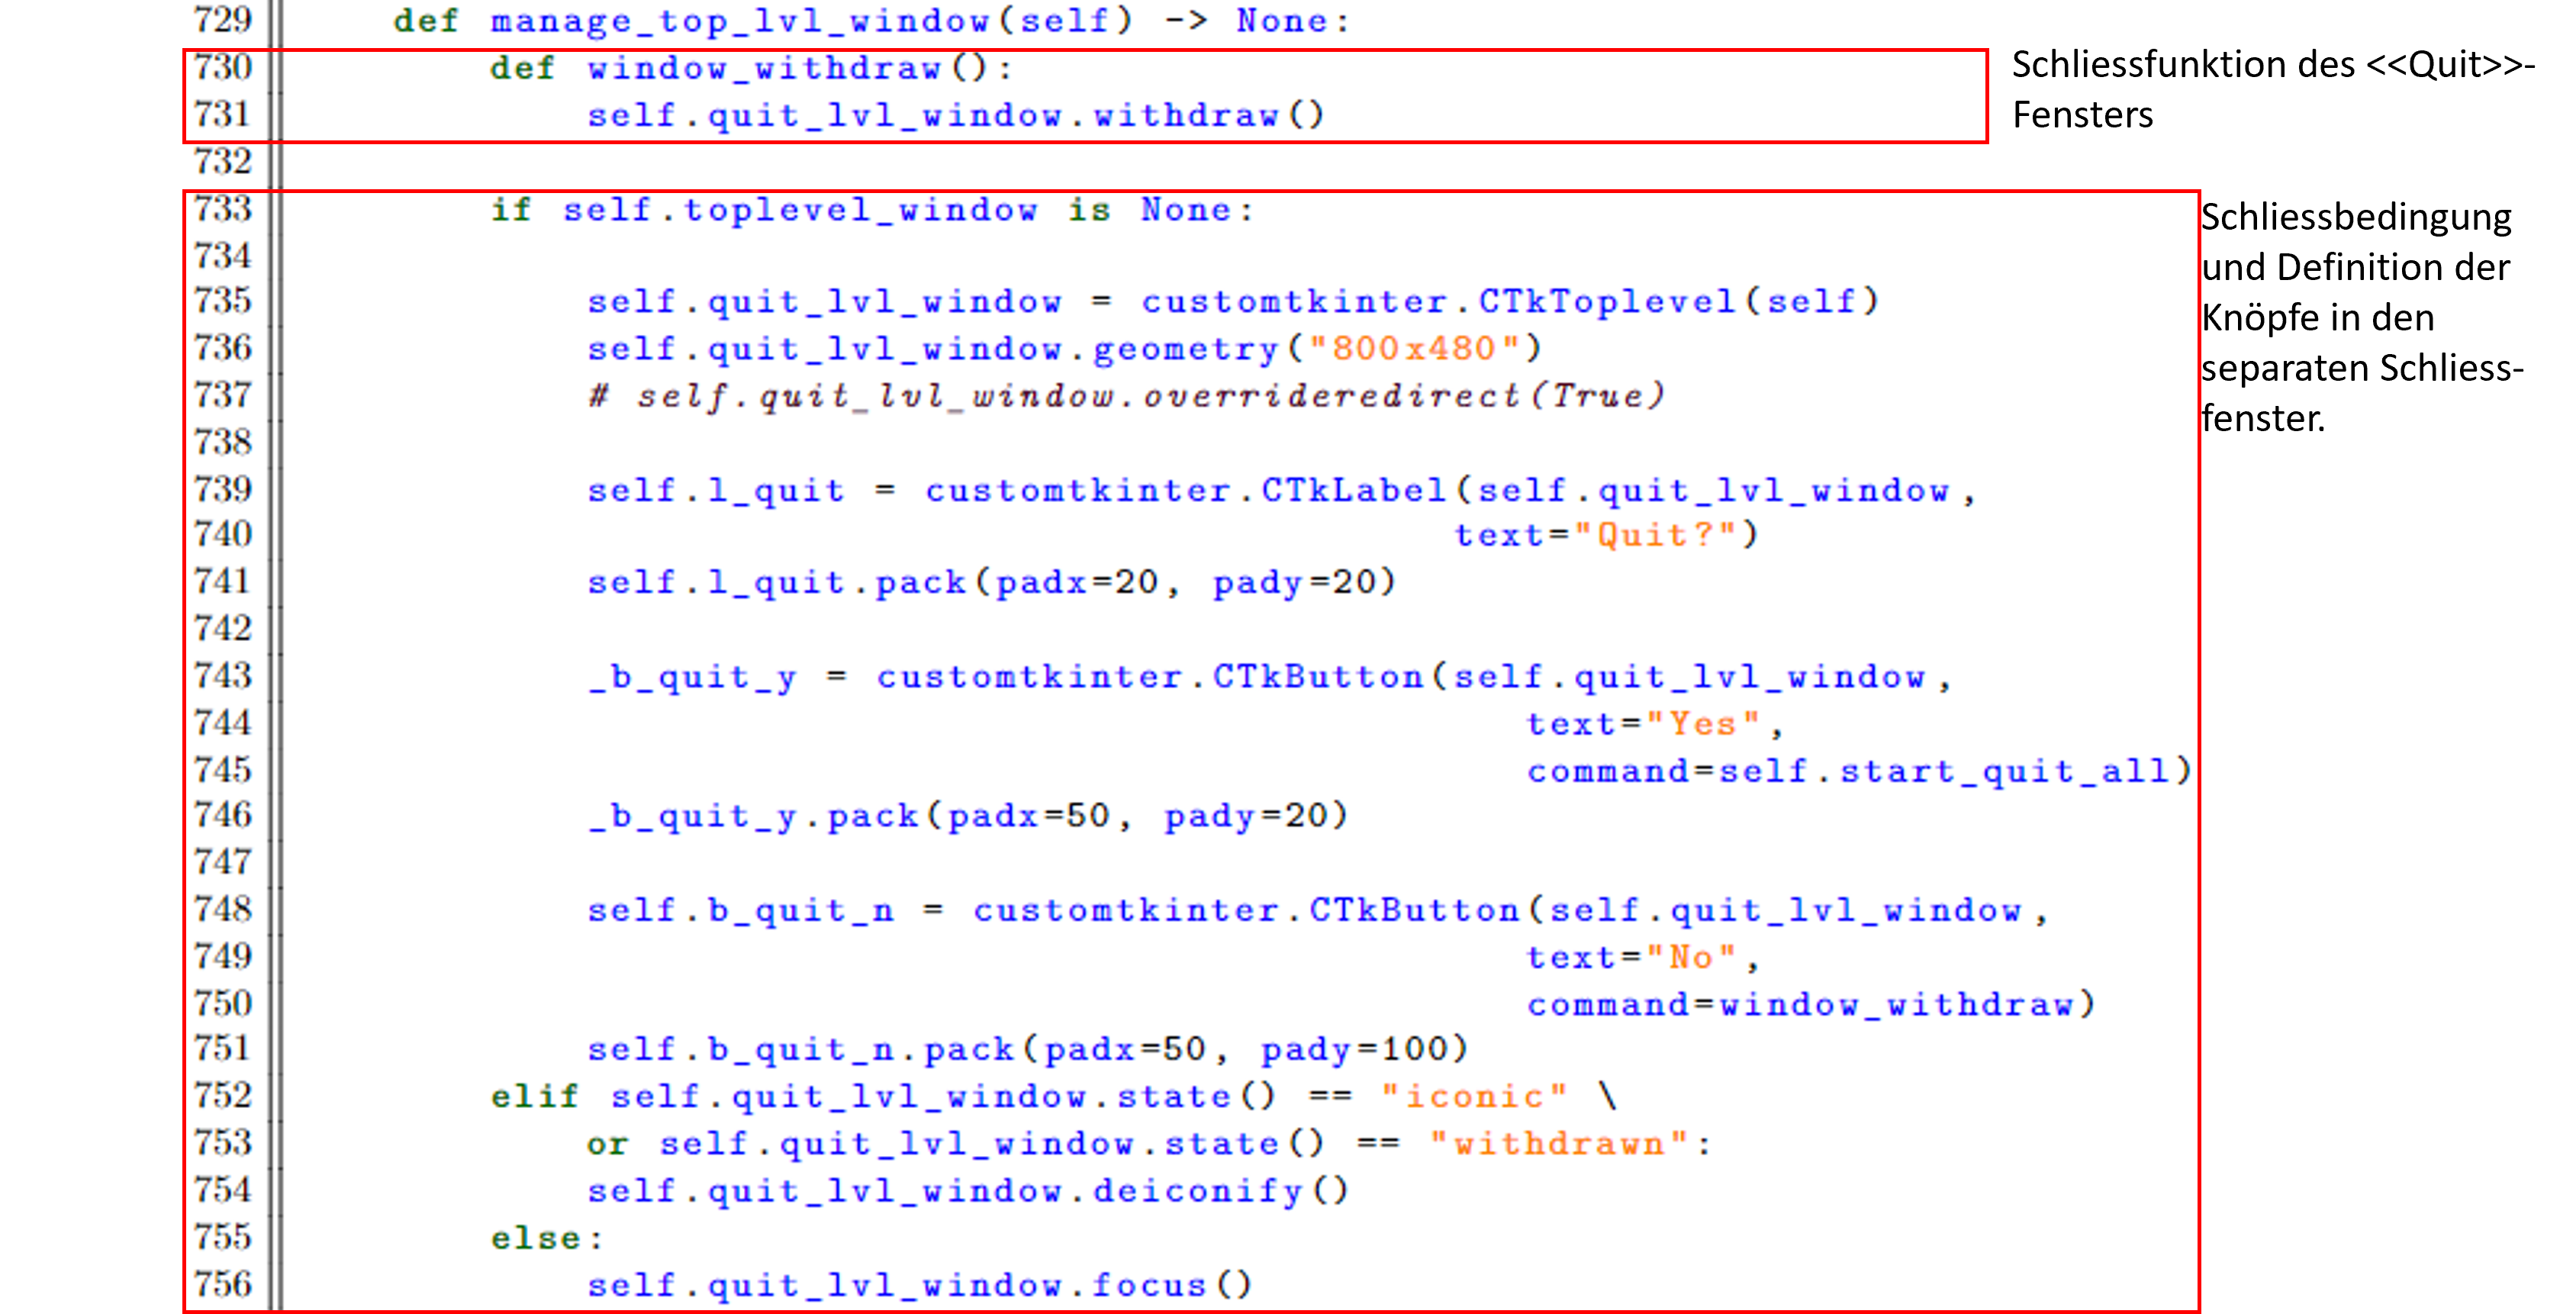
\includegraphics[scale=0.8]{98_images/src/fhnw_pro6m_quellcode_23.png}
    \caption*{Hier wird das separate Fenster für das Beenden erstellt. Für das Herunterfahren der Steuerung schaut die Funktion nahezu identisch aus.}
    \label{fig:fhnw_pro6m_quellcode_23}
\end{figure}

\begin{figure}[H]
    \centering
    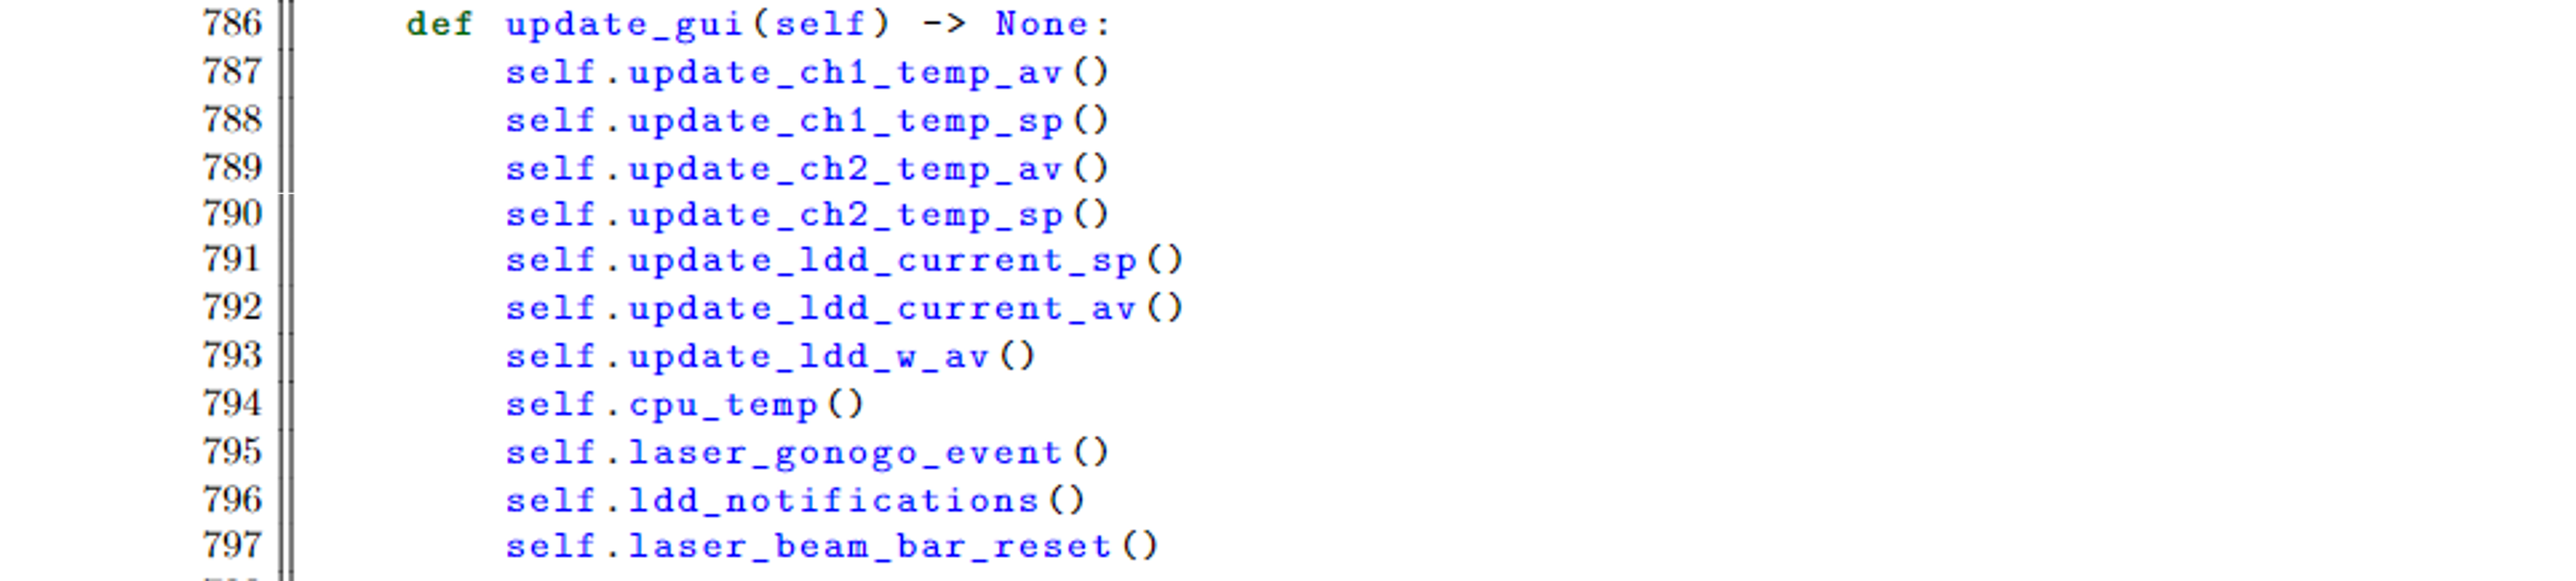
\includegraphics[scale=0.8]{98_images/src/fhnw_pro6m_quellcode_24.png}
    \caption*{Alle Funktionen, die initial gestartet werden sollen, werden in dieser Funktion in einem Thread aufgerufen.}
    \label{fig:fhnw_pro6m_quellcode_24}
\end{figure}

\begin{figure}[H]
    \centering
    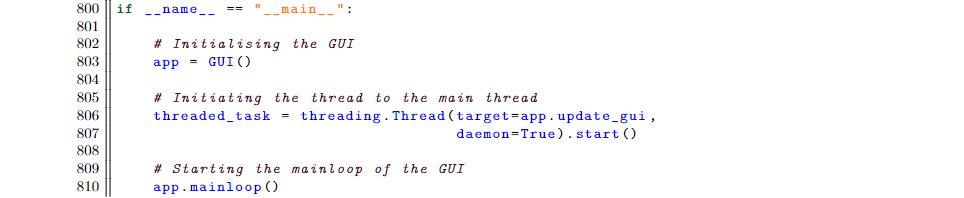
\includegraphics[scale=0.8]{98_images/src/fhnw_pro6m_quellcode_25.png}
    \caption*{Durch die <<if>>-Bedingung startet die Skript nur, wenn genau dieses Skript ausgeführt wird, weil es den Namen <<\_\_main\_\_>> erhält. Die eigentliche Applikation wird mit der Zeile 803 Initialisiert und mit der Zeile 810 gestartet. Zeile 806 startet die in der oberen Abbildung erklärte Funktion zum Starten der initialen Funktionen.}
    \label{fig:fhnw_pro6m_quellcode_25}
\end{figure} 

\subsubsection{Beschreibung des Skriptes <<ldd\_control\_ang.py>>}

\begin{figure}[H]
    \centering
    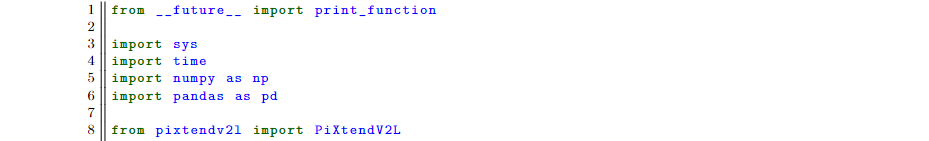
\includegraphics[scale=0.8]{98_images/src/fhnw_pro6m_quellcode_26.png}
    \caption*{Die Importe für den Quell-Code für die Kommunikation mit der SPS.}
    \label{fig:fhnw_pro6m_quellcode_26}
\end{figure} 

\begin{figure}[H]
    \centering
    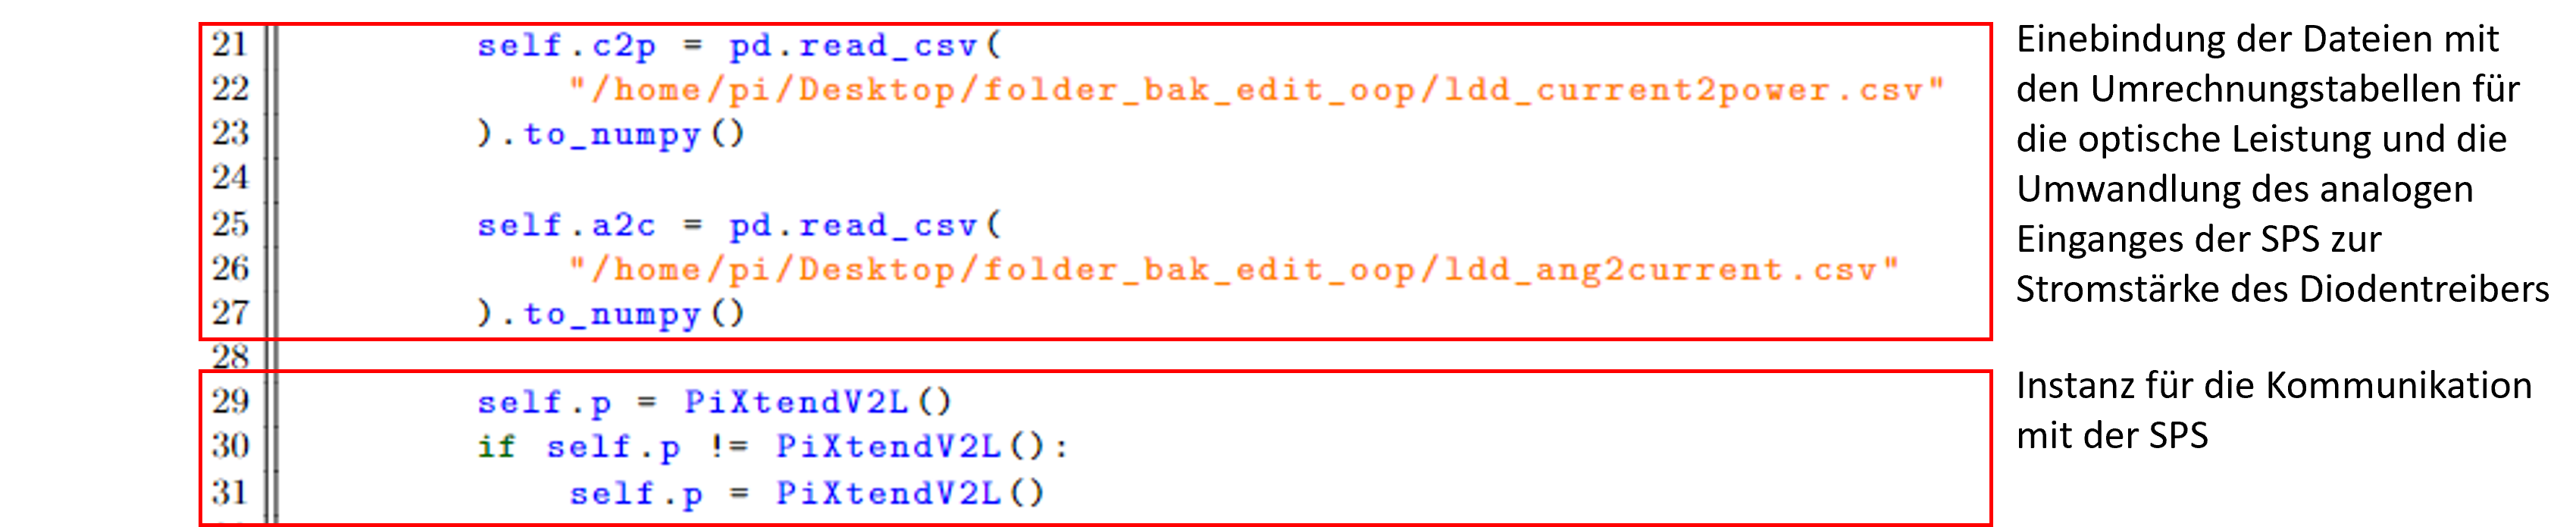
\includegraphics[scale=0.8]{98_images/src/fhnw_pro6m_quellcode_27.png}
    \caption*{Definition der globalen Variablen.}
    \label{fig:fhnw_pro6m_quellcode_27}
\end{figure} 

\begin{figure}[H]
    \centering
    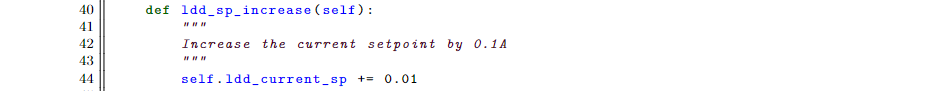
\includegraphics[scale=0.8]{98_images/src/fhnw_pro6m_quellcode_28.png}
    \caption*{Die Funktion für das heraufsetzen der Stromstärke um 0.01A pro Betätigung. Die Funktion für das Herabsetzen funktioniert identisch und wird nicht separat beschrieben.}
    \label{fig:fhnw_pro6m_quellcode_28}
\end{figure} 

\begin{figure}[H]
    \centering
    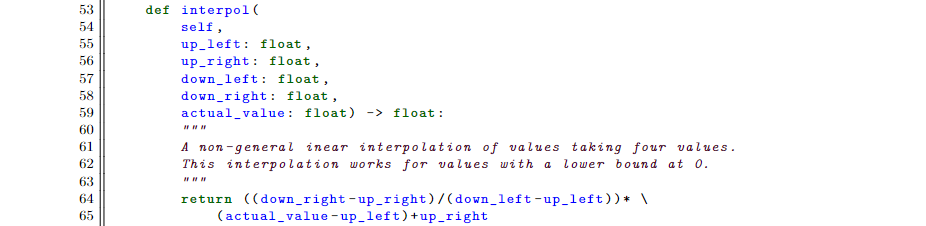
\includegraphics[scale=0.8]{98_images/src/fhnw_pro6m_quellcode_29.png}
    \caption*{In dieser Funktion werden die Stromstärke zum analogen Eingang der SPS und die Stromstärke zur optischen Leistung interpoliert.}
    \label{fig:fhnw_pro6m_quellcode_29}
\end{figure} 

\begin{figure}[H]
    \centering
    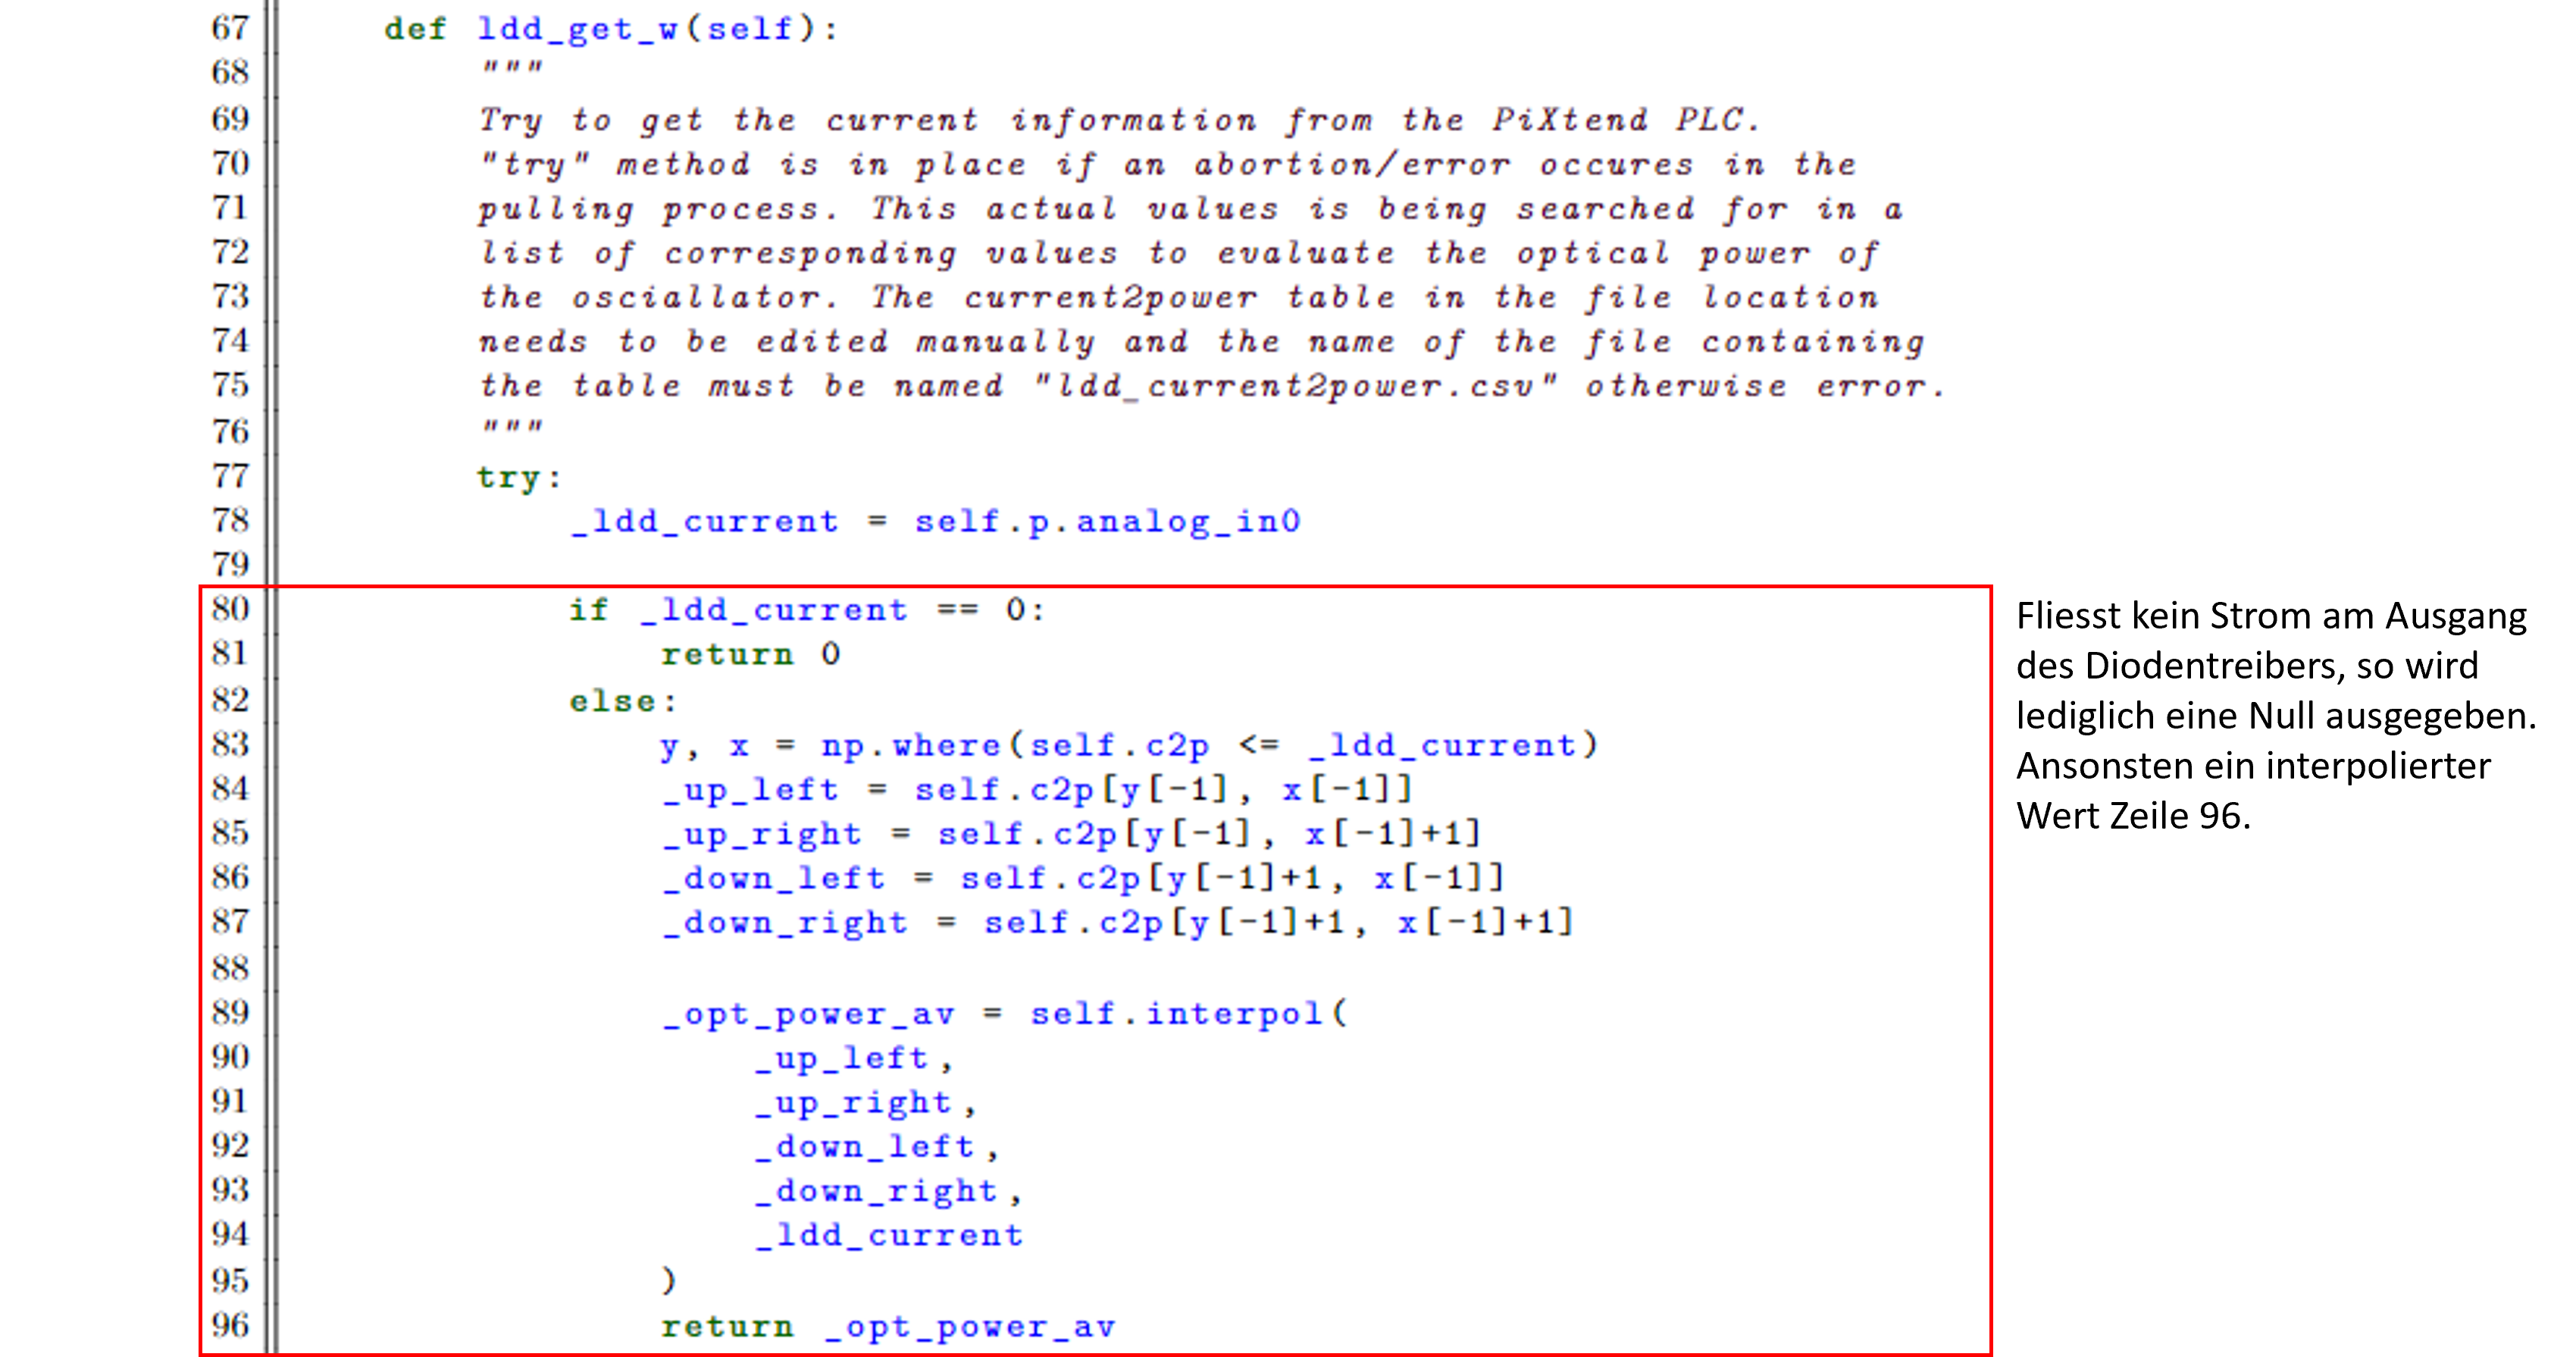
\includegraphics[scale=0.8]{98_images/src/fhnw_pro6m_quellcode_30.png}
    \caption*{Die Funktion versucht den analogen Eingang der SPS zu lesen und reicht den gelesenen Wert zum Weiterfahren an in die Applikation weiter.}
    \label{fig:fhnw_pro6m_quellcode_30}
\end{figure} 

\begin{figure}[H]
    \centering
    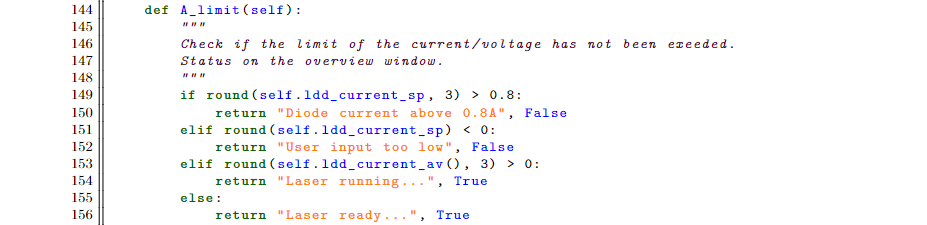
\includegraphics[scale=0.8]{98_images/src/fhnw_pro6m_quellcode_31.png}
    \caption*{Die Statusanzeige des Lasers bezieht hier die Texte anhand von Bedingungen.}
    \label{fig:fhnw_pro6m_quellcode_31}
\end{figure} 

\begin{figure}[H]
    \centering
    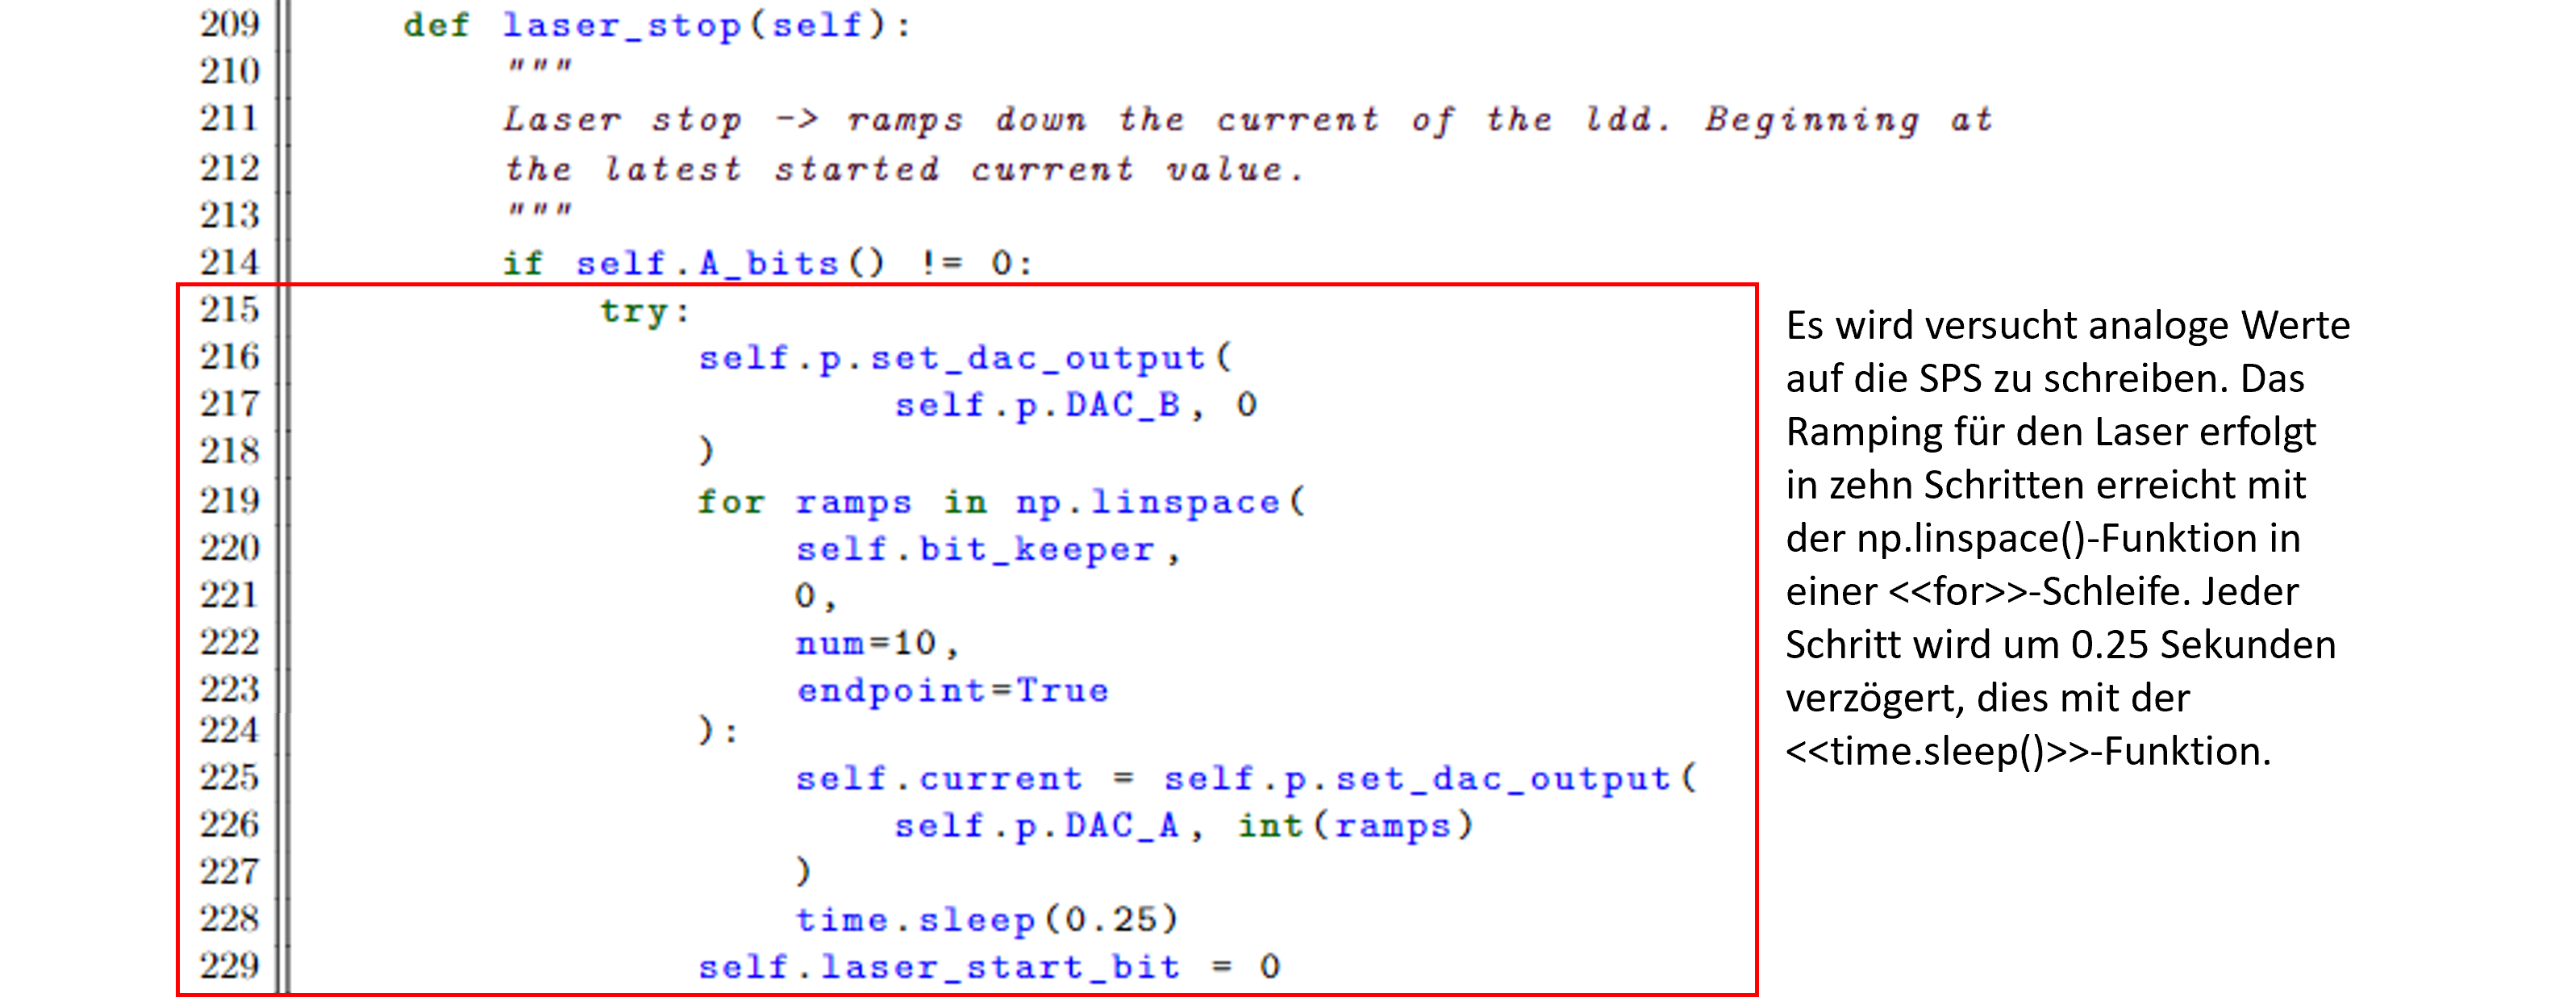
\includegraphics[scale=0.8]{98_images/src/fhnw_pro6m_quellcode_33.png}
    \caption*{Mit der <<laser\_stop>> Funktion wird der analoge Eingang der SPS nach einer Rampe auf den Wert Null gesetzt. Die <<laser\_start>>-Funktion funktioniert identisch.}
    \label{fig:fhnw_pro6m_quellcode_33}
\end{figure}

\subsubsection{Beschreibung des Skriptes <<tec\_control.py>>}

\begin{figure}[H]
    \centering
    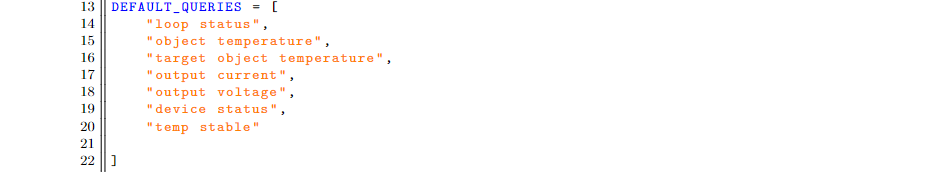
\includegraphics[scale=0.8]{98_images/src/fhnw_pro6m_quellcode_34.png}
    \caption*{Dies ist eine Liste mit Befehlen der API von Meerstetter Engineering.}
    \label{fig:fhnw_pro6m_quellcode_34}
\end{figure} 

\begin{figure}[H]
    \centering
    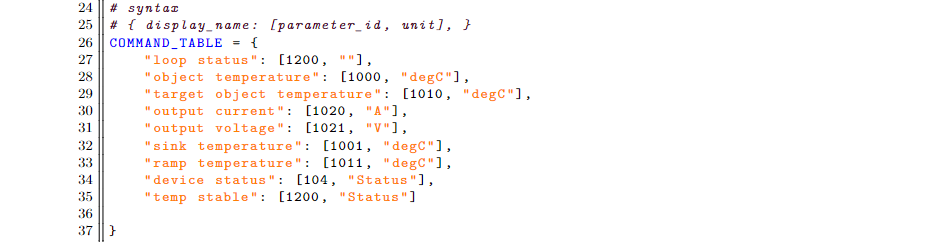
\includegraphics[scale=0.8]{98_images/src/fhnw_pro6m_quellcode_35.png}
    \caption*{Die obigen Befehle werden mit einer Variable des Typs <<dictionary>> mit ganzzahligen Werten versehen, die an den TEC-Kontroller weitergereicht werden.}
    \label{fig:fhnw_pro6m_quellcode_35}
\end{figure} 

\begin{figure}[H]
    \centering
    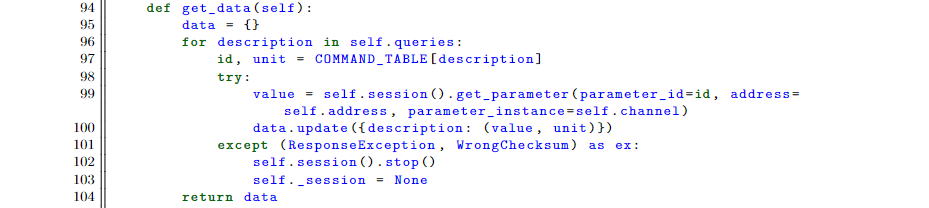
\includegraphics[scale=0.8]{98_images/src/fhnw_pro6m_quellcode_36.png}
    \caption*{Mit dieser Funktion werden mit Hilfe der Befehle aus der obigen Abbildung Daten vom TEC-Kontroller bezogen.}
    \label{fig:fhnw_pro6m_quellcode_36}
\end{figure} 

\begin{figure}[H]
    \centering
    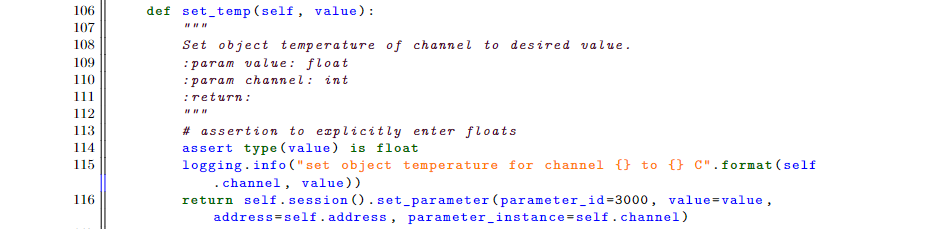
\includegraphics[scale=0.8]{98_images/src/fhnw_pro6m_quellcode_37.png}
    \caption*{Auf die selbe Weise können Daten an den TEC-Kontroller gesendet werden um z.B. Sollwerte zu setzen.}
    \label{fig:fhnw_pro6m_quellcode_37}
\end{figure} 
\end{landscape}

\section{Gesamter Programmcode}
Der Programmcode ist hier in drei Teile aufgeteilt, welche genau so auf dem Raspberry PI aufgebaut sind.\\

\lstdefinestyle{custompython}{
  belowcaptionskip=1\baselineskip,
  breaklines=true,
  frame=L,
  xleftmargin=\parindent,
  numbers=left,
  language=Python,
  showstringspaces=false,
  basicstyle=\footnotesize\ttfamily,
  keywordstyle=\bfseries\color{green!40!black},
  commentstyle=\itshape\color{purple!40!black},
  identifierstyle=\color{blue},
  stringstyle=\color{orange},
}
\subsection{Programmcodes}
\lstinputlisting[caption=Der Haupt-Quell-Code der Steuerung; custom\_gui.py, style=custompython]{gui_custom.py}
\label{main_src}

\lstinputlisting[caption=Der Quell-Code für die Steuerung der SPS; ldd\_control\_ang.py, style=custompython]{ldd_control_ang.py}
\label{ldd_src}

\lstinputlisting[caption=Der Quell-Code für die Steuerung des TEC-Kontrollers; tec\_control.py, style=custompython]{tec_control.py}
\label{tec_src}

\end{appendix}
